\chapter{Preliminaries}
\label{chap:related_work}
This chapter aims to introduce the overarching concepts of glyph-based visualizations. 
The first section provides a grounding on the building blocks of visualizations. 
These blocks are often named as the \emph{visual channels}, of which there are many. 
These are processed by the visual system which we detail in full.
Our visual system and knowledge of how these visual channels are processed forms the basis of concepts such as \emph{pre-attentive processing}, \emph{channel composition}, \emph{global/local features}, \emph{top-down vs bottom-up processing} and so on which are often mentioned in the literature. 
These concepts are important when constructing any visualization since an understanding of how humans process visual information should allow for better visualization design.

The second section introduces glyphs and glyph-based visualization.
We introduce the history of glyphs, their application areas, and finally, their limitations.


\section{The Building Blocks of Visualization}
A visualization is composed of a set of visual items representing pieces of information. 
For each item in a visualization, we may use a number of visual channels\cite{Bertin:1983:book} (referred to Bertin as retinal and planar variables) to represent that item. 
These visual channels are illustrated in Figure \ref{fig:visual-channels}. 
Some channels lend themselves better to some types of data than others, and some channels are perceived better than others.
This section provides an overview of the knowledge about these channels including: 
\begin{itemize}
\item what the visual channels are and when they should be used (semantic relevance); 
\item an overview of current knowledge into how visual channels are processed in the visual system; 
\item the pre-attentive power of visual channels (the pop-out effect); 
\item how these channels are processed in parallel by the visual system;
\item how limits in our visual system limit our capacity to perceive information encoded using different spatial frequencies (\eg, low spatial frequencies for overview, and high spatial frequencies for detailed views) (visual hierarchy); and 
\item which visual channels should not be used together (channel composition). 
\end{itemize}
Better visualizations can be created through better understanding of the primitives available and how best to compose them. 
The end goal of this section is to put in place the foundations to ``encode more important information more effectively'', termed by Mackinlay as the ``Principle of Importance Ordering'' \cite{mackinlay1986automating}.

\begin{figure}[t!]
\centering
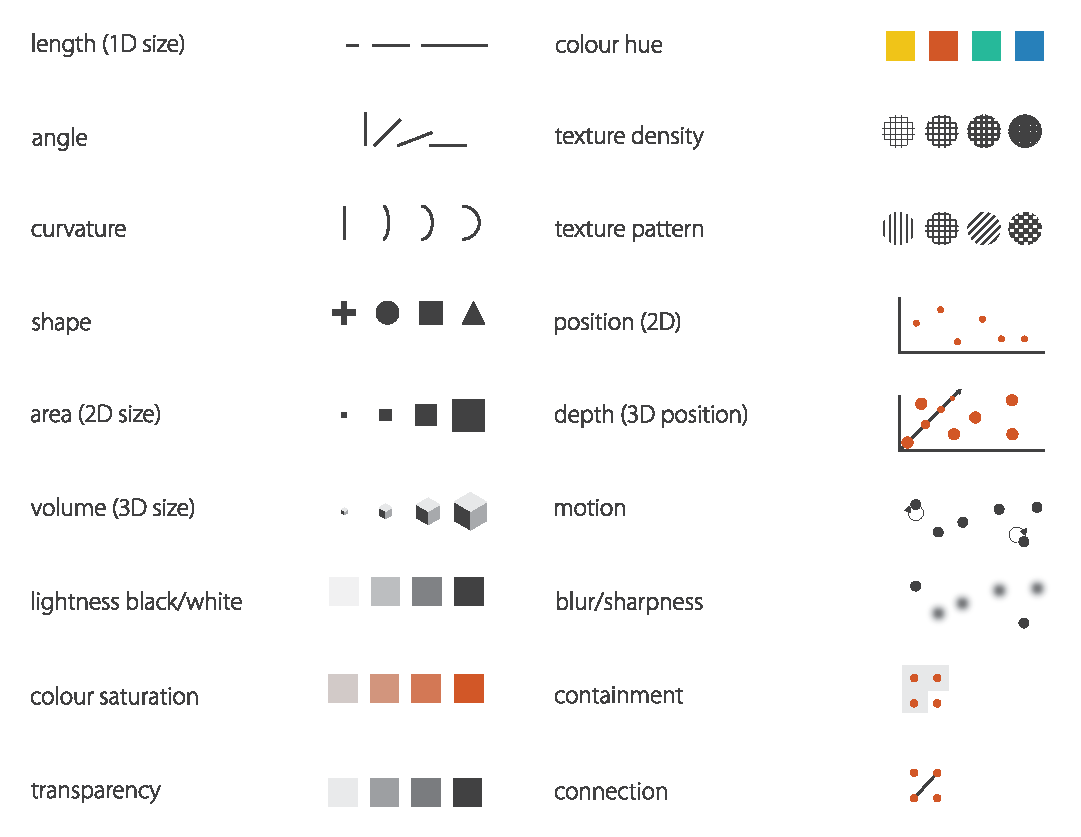
\includegraphics[width=\textwidth]{images/related-work/visual-channels.pdf}
\caption{The types of visual channels available for encoding information from Bertin \cite{Bertin:1983:book} and Ware \cite{ware13}.}
\label{fig:visual-channels}
\end{figure}


\subsection{The Visual Channels and When They Should be Used}
\label{sec:retinal_variables}

This section is organised as follows.
We first introduce the categorisations of visual channels in \ref{sec:viscat}.
This is followed by an investigation of the strengths of visual channels in representing particular types of data in \ref{sec:vispower}.
In \ref{sec:semmapping_vischan} we investigate how semantics can influence the use of particular visual channels.
Finally, in \ref{sec:gestalt}, we introduce Gestalt effects.

\subsubsection{Categorisation of visual channels}
\label{sec:viscat}
Jacques Bertin classified what he termed retinal variables into two categories:
planar (location/position); and 
retinal (size, colour, shape, orientation, texture, and brightness) \cite{Bertin:1983:book,green98}. 
For the sake of consistency, we refer to both retinal and planar variables as \emph{visual channels} throughout this thesis.
Each visual channel has power in representing particular types of data. 
For instance colour could be used to distinguish between male (blue) and female (pink) but it is not as good for representing quantitative data. 
This is also impacted by the cultural association between some colours and more concrete concepts (\eg, blue for male, red for danger, green for go, and so on) \cite{lin2013selecting}. 
Conversely, position can represent quantitative data very well but is not as good as colour for distinguishing between male and female.
The categorisations provided by Bertin were:

\begin{itemize}
\item \emph{associative}: channels facilitating grouping of all elements of a variable despite differing values, \eg, texture, colour, orientation, and shape;
\item \emph{selective}: channels facilitating selection of one category of data, determine the location of visual items with this same category and ignore others, \eg, planar, size, brightness, texture, colour, and orientation variables;
\item \emph{ordered}: channels that facilitate visual ranking of data, \eg, planar, size, brightness, and texture; and
\item \emph{quantitative}: permits extraction of ratios without the need to inspect a legend, \eg, planar and size.
\end{itemize} 

This categorisation is immediately useful since it helps restrict the choice of visual channels depending on the data types that are to be represented. 

\subsubsection{The Power of Visual Channels}
\label{sec:vispower}
What would be more useful are metrics to indicate how the visual channels presented by Bertin are ordered, where the ordering says which visual channels best represent types of information.
So far, metrics are only available to quantify the accuracy of visual channels in representing quantitative data. Stevens \cite{stevens1975} first started measuring the power of variables such as brightness, luminance, length, area, and colour saturation in terms of the stimulus magnitude versus perceived psychological magnitude. 
He found that length was most accurate, with a one-to-one mapping, luminance was perceived greater than intended (1.2), while area and brightness were perceived less than intended (0.7 and 0.5 respectively). 
Performing the worst, colour saturation gave a perceived effect 1.7 times the intended stimulus. 
Stevens found that the majority of stimuli, which included heat, pain, vibration, and duration showed magnified or reduced perceived strength. 
Only length providing one-to-one associations between what the intended stimulus was and how it was perceived. 
A subset of the results from these experiments have been reproduced in Figure \ref{fig:stevens-results}.

\begin{figure}[h!]
\centering
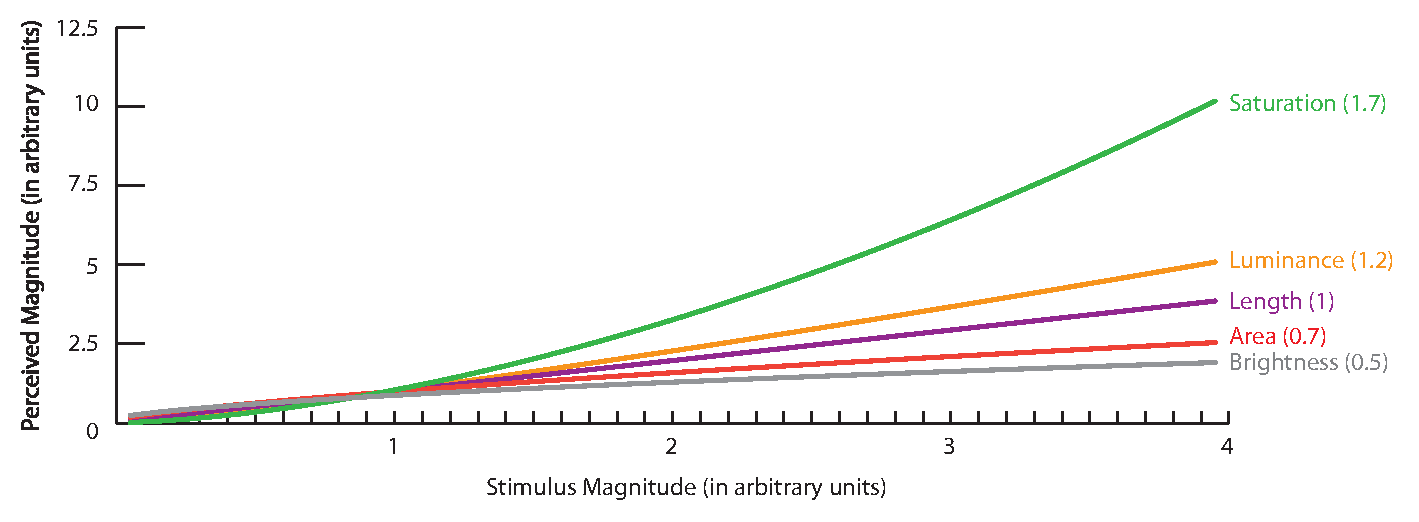
\includegraphics[width=\textwidth]{images/related-work/stevens-psychometrics.pdf}
\caption{A subset of the stimuli and perceived strength versus actual strength by Stevens \cite{stevens1975}.}
\label{fig:stevens-results}
\end{figure}


\begin{figure}[h!]
\centering
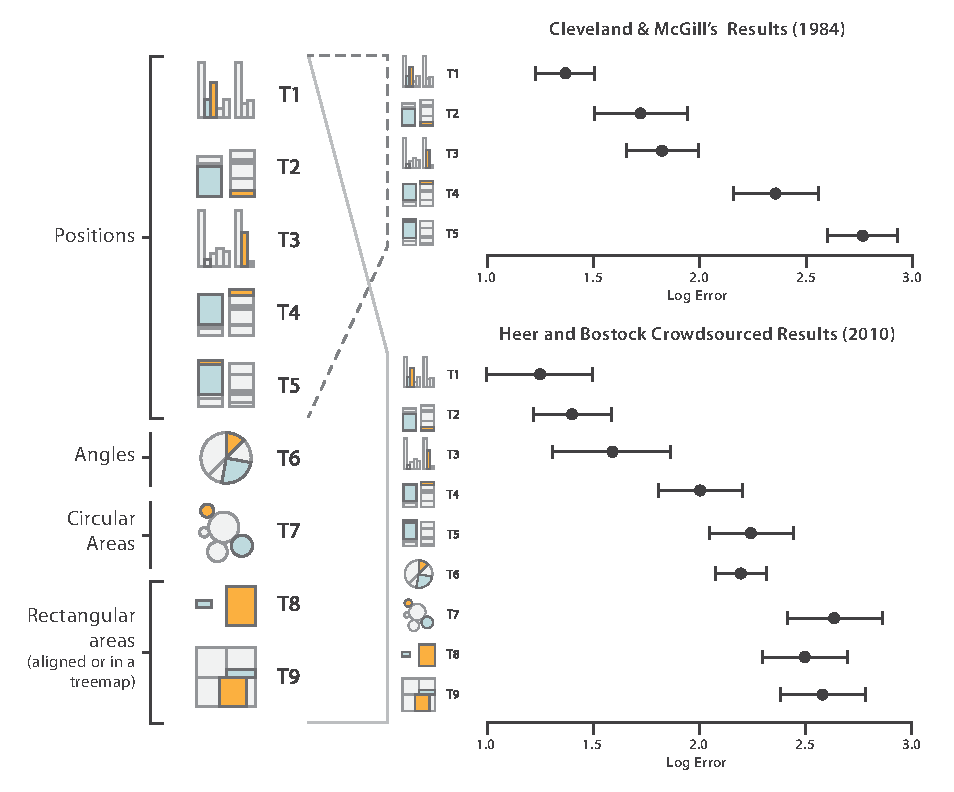
\includegraphics[width=\textwidth]{images/related-work/cleveland_heer_results}
\caption{Observed error rates for different types of visualization using various visual channels to encode the information by Cleveland and McGill \cite{cleveland1984graphical} and Heer and Bostock \cite{heer2010crowdsourcing}. Image adapted from Heer and Bostock \cite{heer2010crowdsourcing}.}
\label{fig:cleveland_heer_results}
\end{figure}

Further to this, research undertaken by Cleveland and McGill \cite{cleveland1984graphical} and recently validated by Heer and Bostock \cite{heer2010crowdsourcing} extended the metrics available for these visual channels as shown in Figure \ref{fig:cleveland_heer_results}. 
This ranking is extrapolated from a series of psychophysics experiments where users are presented with pairwise charts and are asked a series of questions about the underlying data, \emph{e.g.,} what is bigger, A or B. 
The accuracy (and in some cases, response times) for a number of questions are measured. 
For example, in the case of quantitative data, users would be asked what the biggest values are when presented with scatter plots (position), bar charts (length), or bubble charts (area). 
The ``best'' representation is that which obtains the most accurate interpretation from users on average. 

\begin{figure}[h!]
\centering
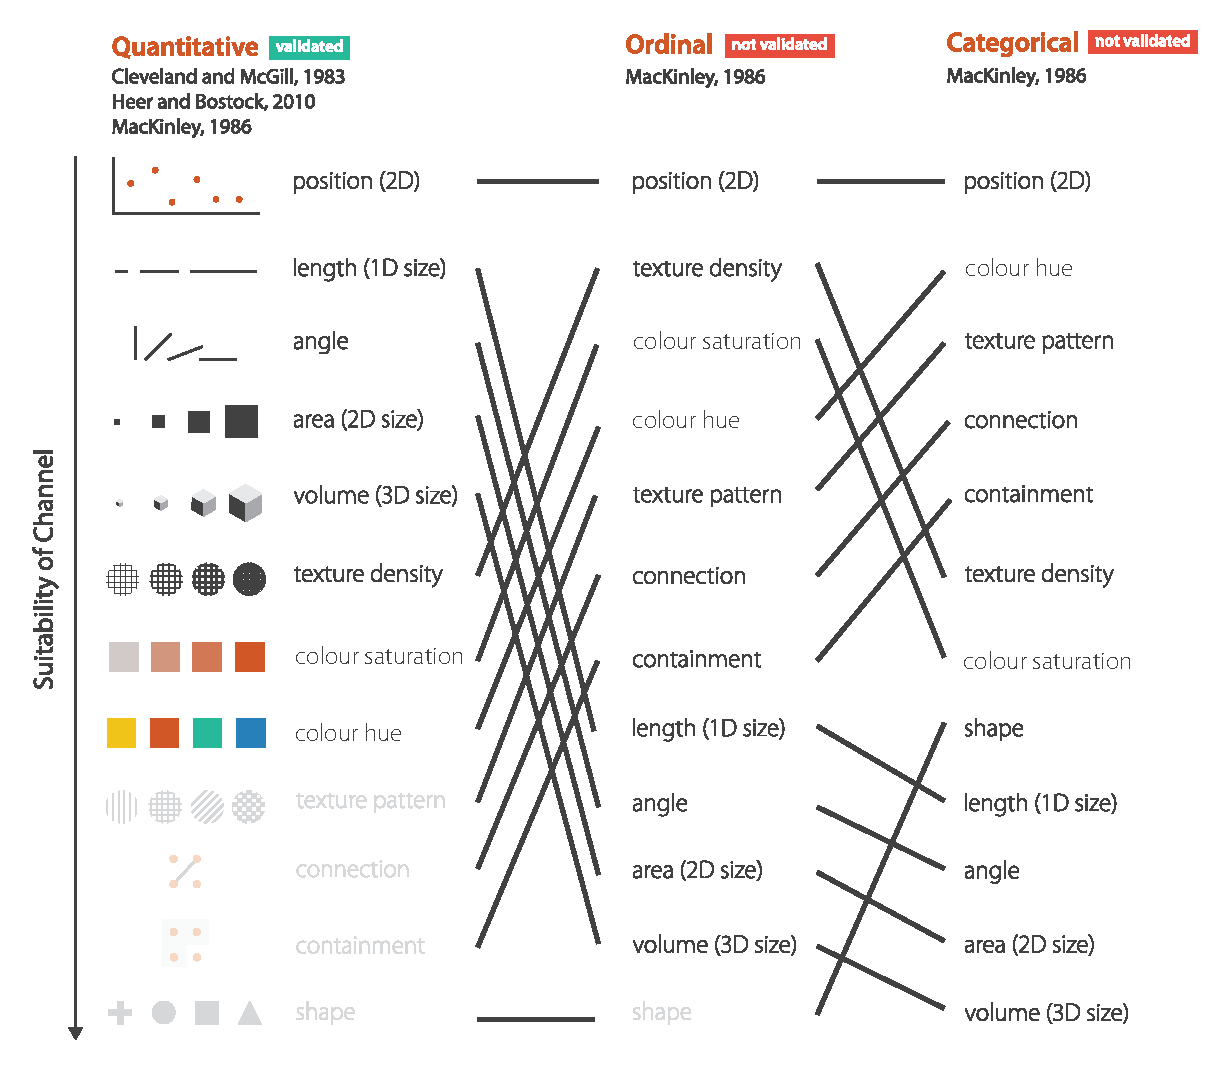
\includegraphics[width=\textwidth]{images/related-work/visual-channel-ordering.pdf}
\caption{A subset of the visual channels from Figure \ref{fig:visual-channels} ordered by MacKinlay\cite{mackinlay1986automating}, Cleveland and McGill \cite{cleveland1984graphical}, and Heer and Bostock \cite{heer2010crowdsourcing}.
Mappings for quantitative visual channels have been validated, however those for ordinal and categorical mappings have not been experimentally validated.
Some visual channels are not applicable to certain data types and these are faded out.}
\label{fig:channel-ordering}
\end{figure}

This ranking was extended to ordinal and categorical data types by MacKinlay \cite{mackinlay1986automating}; however this ranking is not empirically validated, therefore should be taken with a degree of caution. 
Figure \ref{fig:channel-ordering} is derived from \cite{mackinlay1986automating} and serves to represent this ordering, taking note of the fact that ordinal and categorical orderings posed by \cite{mackinlay1986automating} have not been experimentally validated. 

\begin{figure}[h!]
\centering
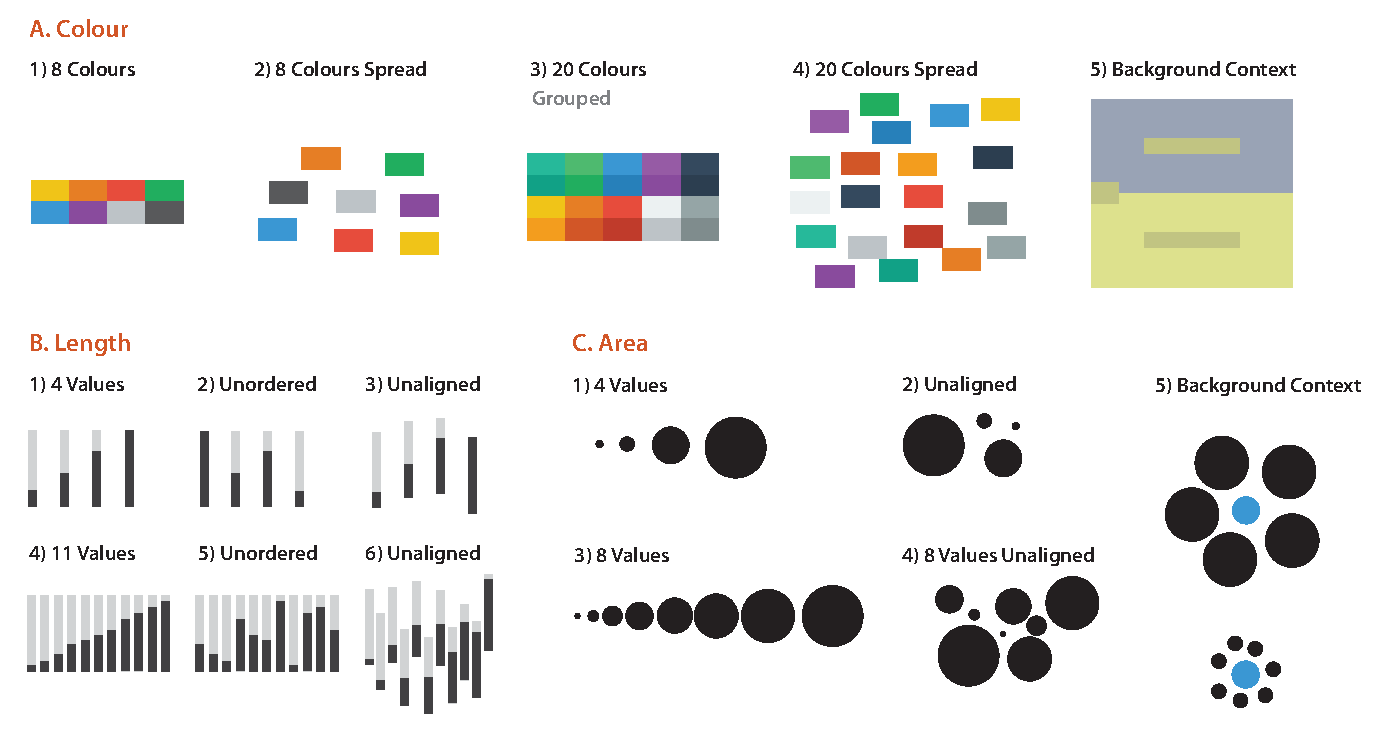
\includegraphics[width=\textwidth]{images/related-work/context-comparison}
\caption{When using various visual channels, we are limited by the number of distinct values we can represent and perceive. Comparison hindered or enabled by the number of values (bins or steps) within each visual channel, their arrangement, and background.}
\label{fig:value-comparison}
\end{figure}

The experiments by MacKinlay and others showed that an accurate interpretation of a value could be made when there exists a sufficiently large distance between the visual elements being compared \cite{mackinlay1986automating, cleveland1984graphical, heer2010crowdsourcing}. 
There are a number of factors that influence comparison:
1) the number of values in the comparison space;
2) the Euclidean distance between those values;
3) the spatial arrangement of the values; and
4) background interference.

Figure \ref{fig:value-comparison} serves to illustrate the contributions these four factors make when comparing different colour hues, lengths, and areas. \\

\noindent\textbf{Colour hues}. It is widely regarded in the visualization community that a visualization should have no more than twelve colours to represent categorical information. 
Having more would make it difficult for the user to distinguish between steps or variations within the limited number of hues available.
Hitt suggested that between no more than five and seven colours should be in a visual display \cite{hitt1992retrofit}. 
Healey validated this statement in an experiment \cite{healey1996choosing}.
Ware proposed a mechanism that divided the hues in to families yielding around eight to twelve distinguishable colours, although this is not experimentally validated \cite{ware13}.
Haroz and Whitney showed how an increase in the number of colours increased response times when finding a target of interest (avoidable through colour grouping\cite{haroz2012capacity}).  

This limitation is illustrated in Figures \ref{fig:value-comparison} A1 and A3 which show two colour maps, one with eight categories, the other with twenty. 
The increased number of categories in Figure \ref{fig:value-comparison} A3 reduces the ``distance'' between the colours. 
Due to the limited number of hues, and the limited number of steps within those hues \cite{ware13}, it becomes more difficult to detect the differences between colours.  
This problem becomes more evident when the grouping of colours is removed in Figure \ref{fig:value-comparison} A4 where some of the greens, oranges, purples, dark blues, and greys look very similar. 
When a user is now asked to perform a visual search task for a hue of orange, he (or she) will find it more difficult to find the orange value amongst the several variations of orange, than one single value of it. 
In addition, colour comparison becomes more difficult when background colour is taken into consideration. 
Due to how the visual system works, and in particular lateral inhibition (which will be discussed later in this chapter), the visual system is continually trying to improve contrast to facilitate edge detection. 
This influences how colours are perceived relative to the background since the brain will dull down one area of an image to make another stand out. 
This causes the classic optical illusion shown in Figure \ref{fig:value-comparison} A5.\\

\noindent\textbf{Length}. Figures \ref{fig:value-comparison} B1 and B4 show how the number of values decreases the perceptual distance between each bar.
The effect is shown with four values which can be perceived well regardless of whether they are sorted or not.
Increasing the number of values results in more data needing to be represented in the same display space.
When sorted, as in Figure \ref{fig:value-comparison} B4, comparing bars is simple.
When unordered in Figure \ref{fig:value-comparison} B5, it is now harder to compare bar height \cite{Chung29112013}. 
When unaligned in Figure \ref{fig:value-comparison} B6, it is very difficult. \\ 

\noindent\textbf{Area}. Figures \ref{fig:value-comparison} C1 and C3 again show how the number of values decreases the distance between visual items. 
When aligned and ordered, comparison is again relatively straightforward, however when unaligned and unordered, the areas in 
Figure \ref{fig:value-comparison} C4 become difficult to compare with numerous areas appearing to be the same size.
Finally, Figure \ref{fig:value-comparison} C5 shows how the background can influence perception of size with two blue circles of the same area appearing to be different due to the size of the surrounding circles.

Consider that in Figure \ref{fig:value-comparison} C5 those blue circles represented the same number of admissions to hospitals in different areas, the bottom blue circle will appear bigger as a result of the surround. 
If other areas have lower admissions, the size of the inner circle will look bigger.
How might that affect policy making, or public perception if shown in a newspaper or TV broadcast where users could not interrogate the visualization for details?

Ensuring there is sufficient visual difference between areas, especially when the task demands accurate comparisons, is imperative to the creation of an effective visualization. 


\subsubsection{Semantic Mapping of Visual Channels}
\label{sec:semmapping_vischan}
Ware \cite{ware2010visual} presents the concept of `semantic mappings' where ``graphical codes''/patterns are inherently related to how humans perceive information in everyday life.
For example, larger objects represent bigger quantities or products closer together in a supermarket are likely to be more similar to each other than objects further away \cite{ware2010visual}. 
In natural language, to reinforce ideas and to help humans build an understanding of hows things are related or positioned, the phrases ``connected to'', ``built on'' or ``contained within'' are used to provide spatial analogies \cite{ware2010visual}. 
In the same way these phrases are used to aid understanding in text, equivalent visual patterns can be used to represent such concepts in visualizations. 
These patterns or ``graphical codes'' are presented by Ware \cite{ware2010visual} and reproduced in Figure \ref{fig:semantic-mappings-ware}. 

\begin{figure}[h!]
\centering
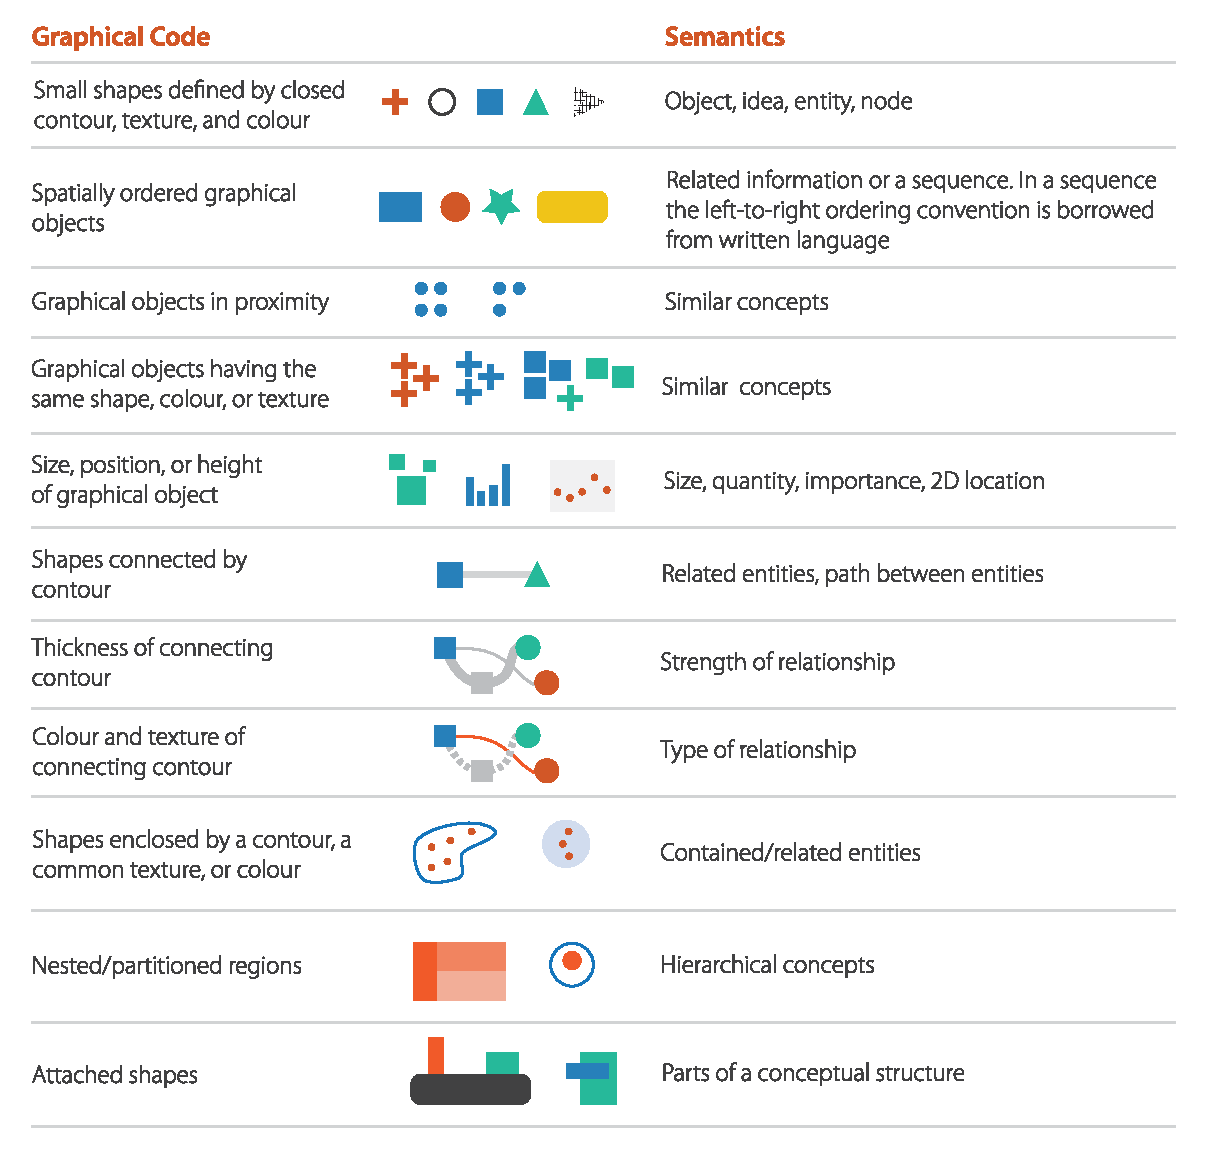
\includegraphics[width=\textwidth]{images/related-work/semantic-patterns.pdf}
\caption{Graphical codes and their semantic mapping. Adapted from \cite{ware2010visual}.}
\label{fig:semantic-mappings-ware}
\end{figure}


\subsubsection{Gestalt Laws}
\label{sec:gestalt}
\begin{chapquote}{Kurt Koffka}{``The whole is other than the sum of the parts.''}
\end{chapquote}


\begin{figure}[h!]
\centering
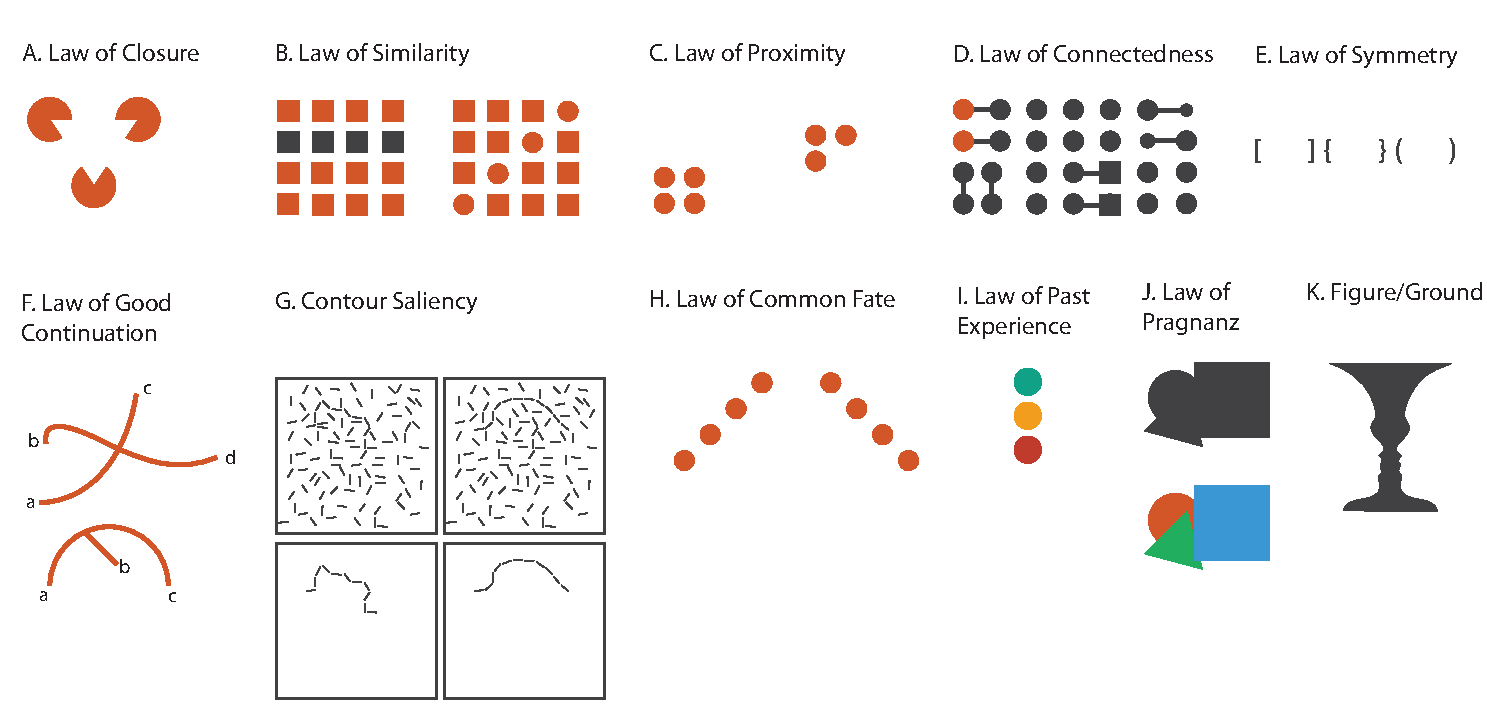
\includegraphics[width=\textwidth]{images/related-work/gestalt.pdf}
\caption{A) \emph{Law of closure} - we look for a single pattern amongst an arrangement of more complex elements. This example shows the Kanisza triangle \cite{ginsburg1975illusory}. 
B) \emph{Law of similarity} - elements with common features are perceived more similar than those that do not have those features. 
C) \emph{Law of proximity} - elements that are closer to each other are perceived more similar. 
D) \emph{Law of connectedness} - connected elements are perceived more related with a stronger effect than colour, shape, size, and proximity. 
E) \emph{Law of symmetry} - we see three groups instead of six individual items. Additionally, the strength of symmetry is greater than proximity. 
F) \emph{Law of good continuation} -  lines are linked when collinear - \textbf{a} and \textbf{c} and \textbf{b} and \textbf{d} in the top example appear as one as does \textbf{a} and \textbf{c} in the bottom image. However \textbf{a} and \textbf{b} do not appear to belong to the same line (adapted from \cite{kandel2012principles}). 
G) \emph{Contour saliency} - smooth contours can be perceived more easily than a jagged contour (adapted from \cite{kandel2012principles}). 
H) \emph{Law of common fate} - groups of items going towards a particular direction are perceived as one. Here, two groups can be perceived. 
I) \emph{Law of past experience} - our experiences have an impact on how we perceive often abstract items. In this example, with three ellipses coloured green, amber and red, we perceive a traffic light although the intention of the designer may have been different. This is a common factor with colour where different colours in different countries mean different things. 
J) \emph{Law of Pragnanz} - this refers to the brain's preference to split complex objects in its simplest constituent parts.
K) \emph{Figure/Ground} - the visual system processes parts of the image as the main object of interest (figure) and the rest as the background (ground).}

\label{fig:gestalt}
\end{figure}

Many of these graphical codes are derived from \emph{Gestalt} psychology, translated from German to mean ``configuration or form'' \cite{kandel2012principles}. 
\emph{Gestalt} psychologists posed the theory that a visual system processes sensory information about the colour, distance, form, and motion of objects through the application of a set of rules. 
This theory gave rise to a number of ``Gestalt laws'', specifying how certain configurations of objects, \eg, proximity, similarity, good continuation, closure, connectedness, common fate, familiarity, and symmetry play into our perception of the world around us. 
These laws are illustrated in Figure \ref{fig:gestalt} and are formed through the observation of four key points:

\begin{itemize}
\item \textbf{Emergence} - the whole object is identified ahead of its constituent parts; that is, we will look at the outline of an object and match these outlines to what we already know then identify the rest of the smaller parts.
This refers to global-local processing and is discussed more in Section \ref{sec:global_local_processing};
\item \textbf{Reification} - our ability to fill in the gaps as in Figure \ref{fig:gestalt} A;
\item \textbf{Multi-stability} - is illustrated in the figure/ground example in Figure \ref{fig:gestalt} K which shows the stable/unstable depiction of what is figure and what is ground. 
We can see the two faces or a vase depending on whether or not you see the black as the figure or ground. 
The ability to go between the vase and the two faces makes the relationship unstable; and
\item \textbf{Invariance} - the innate ability of our visual systems to identify items with a tolerance for change allows our visual system to recognise a square even if its rotated or slightly distorted or a face even if viewing a profile and not the frontal view.
\end{itemize}


\section{The Visual System}
\label{sec:vis-processing}

\begin{chapquote}{Richard L. Gregory, Eye and Brain, 1966}{``We are so familiar with seeing, that it takes a leap of imaginations to realise that there are problems to be solved. But consider it. We are given tiny distorted upside-down images in the eyes and we see separate solid objects in surrounding space. From the patterns of stimulation on the retina we perceive the world of objects and this is nothing short of a miracle.''}
\end{chapquote}

\emph{``How do we see?''} has been a question behind a large body of research for many decades and scientists are still trying to answer it. 
There is no complete model describing the complete visual system in terms of how we go from vision to understanding.
However, there is a great deal of validated research into the building blocks of visualization and how various visual channels introduced earlier are processed by our visual system.
This research is based largely on experiments performed on animals (\eg, cats by Hubel and Wiesel in 1958 \cite{hubel1959receptive}), and later in primates, whose visual system is largely homologous with that of humans. 

This section presents an overview of the basic principles of visual processing, with a focus on details relevant for visualization design.
Acting as a primer for discussions around pre-attentive processing, channel separability, and visual hierarchy, this section presents an overview of the basic principles of visual processing.
This encompasses research on how the visual system is physically arranged, how a visual scene is decomposed into its constituent parts (local areas of contrast), then recomposed by the visual system.

Three coordinated and cross-interacting processes detailed below are imperative to the visual system, extending from the eyes through to the visual cortex at the rear of the brain:  
\begin{itemize}
\item \textbf{Low-level processing} - at this level of processing, visual primitives, those being colour, local contrast, orientation, binocular disparity (different images of the same scene from each eye) for 3D depth perception, and movement are processed \cite{kandel2012principles}.
This will be described below in more detail and relies on cells in the retina, the lateral geniculate nucleus, and the primary visual cortex (V1) and V2 at the rear of the brain;
\item \textbf{Intermediate-level processing} - here, the scene is analysed given the visual primitives obtained at the previous level of processing to perform contour integration, identify object boundaries, analyse surface properties, depth and segmentation, determine object motion, and what is the figure versus the ground \cite{kandel2012principles}.
\item \textbf{High-level processing} - in the \emph{ventral stream} (what pathway) for object identification based on contours, surfaces, movement, and depth found in the visual processing stages in combination with past experience; and the \emph{dorsal stream} (where pathway) for motion detection and guidance of movement in the 3D world.
\end{itemize}

\subsection{Low-level Processing}
Low-level processing starts in the retina. 
When we process a visual scene, the rods (achromatic sensitivity) and cones (chromatic sensitivity) become activated by light photons with the result being the inhibition of release of a neurotransmitter called glutamate which normally moves across a synapse onto what are called bipolar cells. 
Cones are linked to two types of bipolar cells (ON/OFF) whereas rods have only one type of bipolar cell. 
ON bipolar cells are inhibited (hyperpolarised) by the presence of glutamate and OFF bipolar cells are excited (depolarised) by glutamate. 
When glutamate stops being released from the photoreceptor, the ON bipolar cell becomes more depolarised and the OFF bipolar cell less depolarised. 

Rods synapse with a special type of bipolar cell that interact with cells named amacrine cells (not ganglion cells as is the case for cones). 
These amacrine cells create a horizontal connection which enables lateral inhibition of the bipolar cells connected to cones. 
The horizontal connections help in creating visual acuity through inhibition of the less illuminated areas of a receptive field, where 
less well-illuminated areas have their signal reduced leaving the more-enhanced illuminated areas. 
This results in better contrast between the better and less well-illuminated areas in the visual field. 

There are many more photoreceptors in the retina than there are axons (~1\% of total receptors) in the optic nerve to represent them \cite{kandel2012principles}. 
Therefore, the first levels of visual processing occur directly in the retina through comparison and aggregation of photoreceptor outputs. 
At this point in the visual system, this comparison and aggregation occurs to help in detecting local contrast (for edge detection). 
To achieve this, one retinal ganglion cell compares and summates the responses of a varying number photoreceptors, with the number of photoreceptors directly related to the proximity of the photoreceptors to the fovea. 
This relationship between a retinal ganglion cell and the photoreceptors associated with it is termed the \emph{receptive field of the ganglion cell}. 
The receptive fields can be categorised into two main types, \emph{on-centre} and \emph{off-centre} which are illustrated in Figure \ref{fig:receptive-fields}. 
These fields allow for detection of contrast since they are selective for differences in illumination, and therefore contours/edges in the image \cite{kandel2012principles}. 
A smaller receptive field near the fovea allows for discrimination of fine detail (high spatial frequencies) and larger receptive fields towards the periphery are tuned for more coarse details (low spatial frequencies). 
Additionally, motion is shown to elicit a stronger response in the ganglion cells than a non-moving object \cite{kandel2012principles}. 

\begin{figure}[t!]
\centering
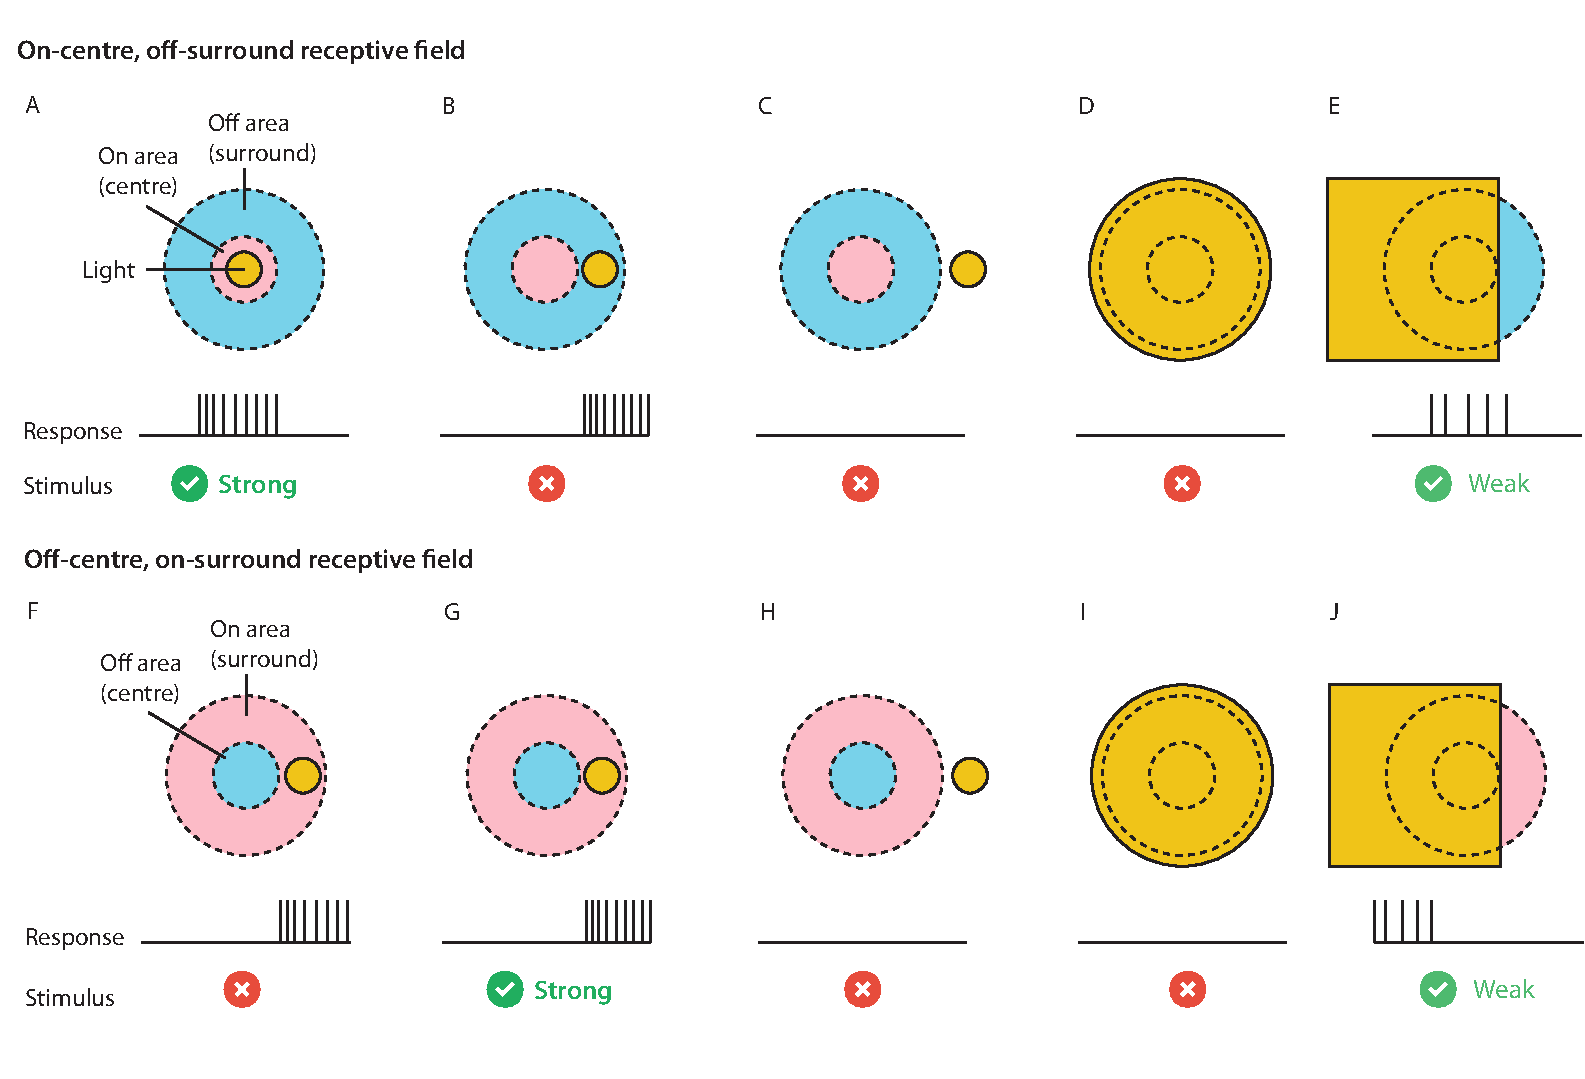
\includegraphics[width=\textwidth]{images/related-work/receptive-field}
\caption{Two types (\emph{on centre and off centre}) of receptive fields stimulated under five conditions. 
A) The response of the ganglion cell's receptive field is strongest when the light is shown directly in the centre. 
The response would be the opposite for an \emph{off-centre, on-surround} receptive field as shown in F. 
B) Light shone on the surround area causes a response in the receptors, however there is no stimulus recorded due to the selectivity of the cell. This is the opposite in the \emph{off-centre, on-surround} as shown in G. 
C) and H) Light outside the receptive field obviously records no stimulus in both types of receptive field. 
D) and I) When light covers the whole field, there is no response recorded at all - this shows how this type of cell is selective for contrast. 
E) and J) Weak responses are generate when the receptive field is partially covered by light.} 
\label{fig:receptive-fields}
\end{figure}

\begin{figure}[h!]
\centering
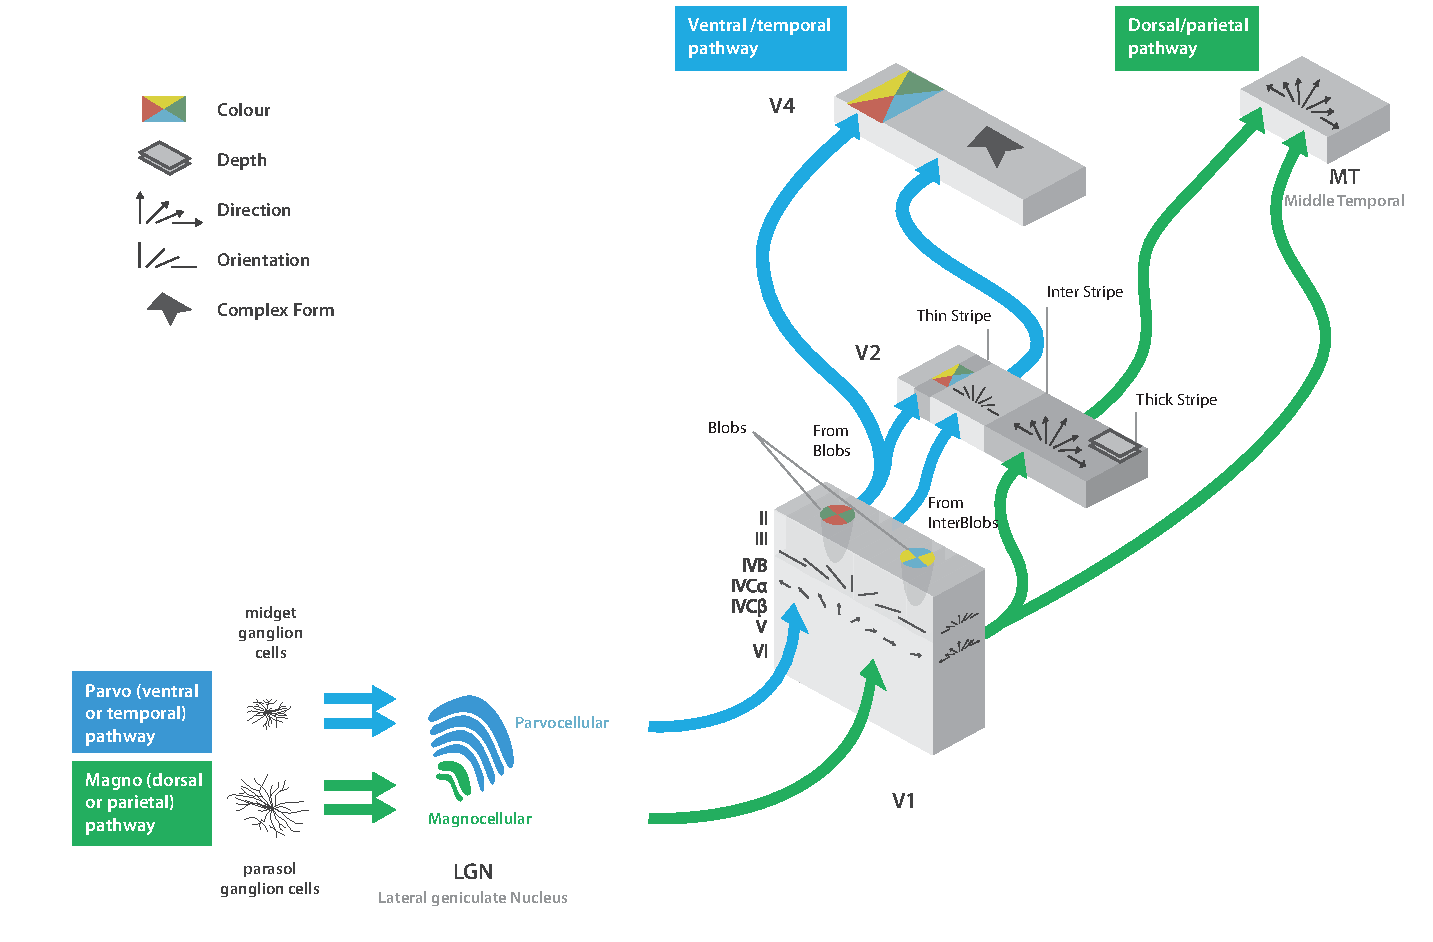
\includegraphics[width=\textwidth]{images/related-work/parallel-processing-visual-pathways}
\caption{Parallel processing in visual pathways adapted from Kandel \etal, 2012 \cite{kandel2012principles}. 
Object identification is conducted in the ventral stream through cells selective for form and colour information. 
Visually-guided movement is performed in the dorsal stream with use of movement sensitive cells. 
There is significant interconnectivity between these two pathways.}
\label{fig:visual-processing}
\end{figure}


Retinal ganglion cells exist in three main forms in primates, as M (magno)-, P (parvo)-, and K (koniocellular)-ganglion cells.
M and P ganglion cells are spatio-temporal filters that feed into two parallel pathways in the visual system (magno and parvo) \cite{merigan1993parallel}.
M cells do not select for colour, but have a greater sensitivity to rapidly moving stimuli \cite{merigan1993parallel}.
P cells have greater spatial resolution, selectivity for colour, and the ability to respond to slowly changing or slowly moving stimuli \cite{merigan1993parallel}.
K cells are interspersed between M and P ganglion cells and are said to be involved in relaying colour information and low resolution details to V1 \cite{hendry2000koniocellular}.
Figure \ref{fig:visual-processing} shows a simplified view of how input comes from the LGN in to the visual cortex via a parallel stream with object recognition facilitated by the parvo pathway, and visually guided movement facilitated by the magno pathway.
Communication occurs along these pathways via signals aided by the firing of neurons (action potentials).
These signals pass along the optic nerve, through the optic chasm, down the optic tract, into the lateral geniculate nucleus (LGN) which also contains contrast processing cells, to the optic radiation, and finally into the visual cortex.
This model is often used to illustrate the visual system, however there is evidence to suggest that the magno and parvo pathways have significant flow of information between them \cite{merigan1993parallel}.
Location information is preserved from the retina in what is called a retinotopic map, a direct mapping between an area in the retina and its respective processing area in the LGN and visual cortex.

Moving from the LGN to the visual cortex there is a change in the structure of the receptive fields which represents a shift in the type of visual processing occurring within the visual system.  

The primary visual cortex is presented as a columnar arrangement of neurons sensitive to orientation \cite{hubel1959receptive}, direction, and colour-sensitive neurons (blobs with small circular receptive fields) \cite{horwitz2012nonlinear} interspersed regularly across the structure (Figure \ref{fig:visual-processing}). 
This columnar structure features right and left eye dominant columns that alternate every 750-1000$\mu$m alongside criss-crossed columns selective for particular orientations \cite{horton1984mapping}. 
Orientation-selective neurons are split into two types: simple; and complex. 
Simple neurons have ON and OFF subregions where if there a bar of light of a particular orientation enters the ON region, the neuron fires. 
The neuron also fires when the bar leaves the OFF region. 
Complex neurons on the other hand fire continuously as the bar moves across its receptive field. 
These neurons were first discovered by Hubel and Wiesel in 1958 in experiments performed on the cat \cite{hubel1959receptive} and are illustrated in Figure \ref{fig:orientation-cells}. 
They are thought to be arranged into what are termed \emph{hyper-columns} representing the populations of neural cells selecting for specific orientations in the full 180$^{\circ}$ of possibilities. 
These hyper-columns are thought to repeat across the visual cortex every 750$\mu$m.

\begin{figure}[t!]
\centering
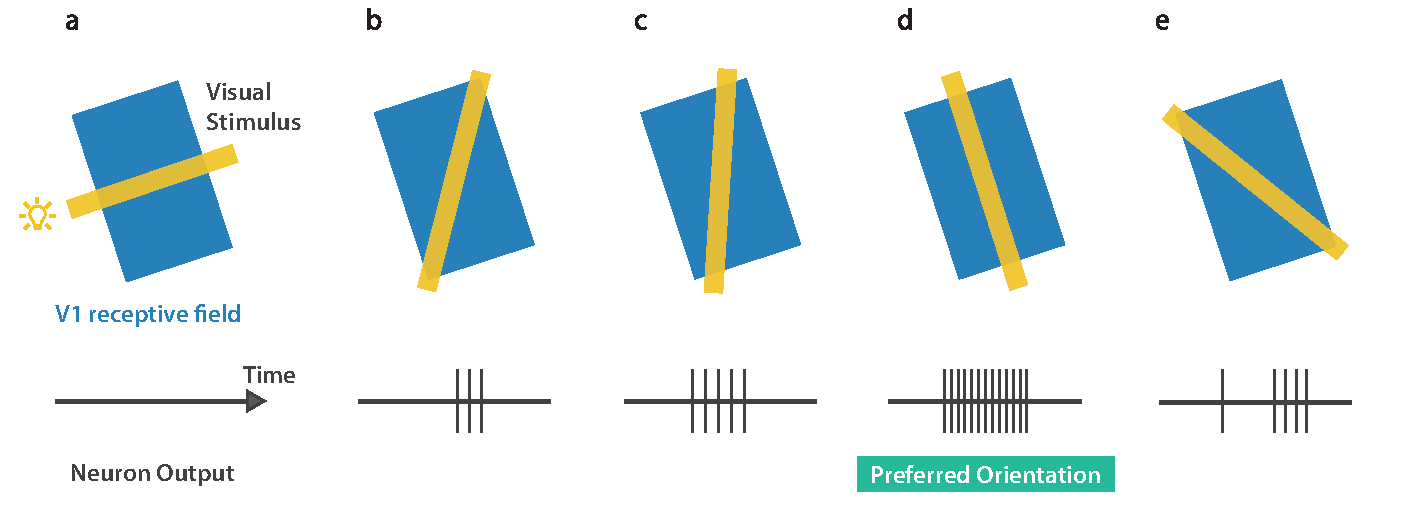
\includegraphics[width=\textwidth]{images/related-work/orientation.pdf}
\caption{A receptive field (blue) and the neural response to a flashing light bar stimulus (yellow). 
The examples show how specific neurons have distinct preferences for orientation with a) performing worst and d) providing the strongest response. 
Adapted from \url{http://neuroscience.uth.tmc.edu/s2/chapter15.html}.}
\label{fig:orientation-cells}
\end{figure}

As illustrated in Figure \ref{fig:orientation-cells}, these neurons will fire whenever presented with a stimulus, in this case a bar of light with a particular orientation. 
This means that for every position in the retinotopic map, if there is contrast, these positions will be converted into local contours.
These local contours are thought to be the basis of shape and surface detection in the intermediate-level processing stage which will be detailed further below.\\

\subsection{Intermediate-level processing}
Intermediate-level processing involves convergence of the many line segments and surface properties detected in low-level processing and the construction of complex patterns and objects. 
This process is thought to involve: contour integration; identification of object boundaries and therefore identification of the figure versus ground; object motion; and analysis of surface properties, depth, and segmentation. 
A key property of the cells involved at these stages of visual processing is the widening receptive field to capture overall details of many smaller parts (\eg, local contours or local regions of surface change).

\subsubsection{Contour Integration}
As illustrated in Figure \ref{fig:gestalt} G, Gestalt laws state that smooth contours are more salient (they ``pop-out'') when compared to more jagged contours.
This may be explained by horizontal connections that exist between columns with similar orientation preferences in area V1 of the visual cortex \cite{kapadia1995improvement}. 
Therefore when a straight line is observed in one column, a preference is enforced via horizontal connections for columns with a similar orientation \cite{kapadia1995improvement}.
This mechanism could enforce a preference for continuity (smooth lines). 

Next, there is \textbf{identification of object boundaries} also referred to as figure/ground discrimination \cite{lee2003computations, qiu2005figure} or border ownership (BOWN) which is said to occur largely in V2. 
We see a three-dimensional (3D) world even though our eyes capture a two-dimensional (2D) scene. 
To be able to infer depth as the third dimension we must look at many visual cues such as shadows, occlusion, differences between both eyes (binocular disparity), and previous knowledge to determine how the three dimensional world is arranged. 
So how does one object relate to another? Is an object the figure or is it the ground? 

There are two competing theories of how the visual system computes this. 
The first is by Lamme \cite{lamme1995neurophysiology} who was the first to find that some neurons fired more frequently to objects in a figure region as opposed to objects in the ground region. 
He proposed that regions in a scene are labeled (region labelling), with closer (occluding) regions labeled the figure, and the further away (occluded) region labeled as the ground.

The second theory by Zhou \etal \cite{zhou2000coding} proposed a more complex model where different regions can be labeled with relative depth orderings followed by border ownership processing. 
The more plausible theory is that put forward by Zhou \etal \cite{zhou2000coding} due to its power in explaining complex figure/ground scenarios such as the previously-mentioned Rubin's vase/faces illusion. 

Qiu \etal \cite{qiu2005figure} built on the work by Zhou \etal \cite{zhou2000coding} to show that area V2 in the macaque monkey employed two computational strategies for establishing the figure from ground. 
One strategy determines local depth order through exploiting binocular stereoscopic information \cite{qiu2005figure}. 
The other exploits Gestalt factors such as closure available through processing the global arrangement of contours\cite{qiu2005figure}. 
Figure \ref{fig:bown} shows a number of examples of the border ownership problem where in Figure \ref{fig:bown} C the figure is considered to be the orange ellipse but when the perspective is changed, the blue shape becomes the figure. 
In each case, ownership of the border is assigned to different objects reflecting their position in 3D space. 
Figure \ref{fig:bown} also depicts what are interactions between BOWN cells using green dotted lines. 
This messaging system is said to excite BOWN cells that are in agreement and inhibit BOWN cells in disagreement to create a depth map with all possible combinations. 

\begin{figure}[t!]
\centering
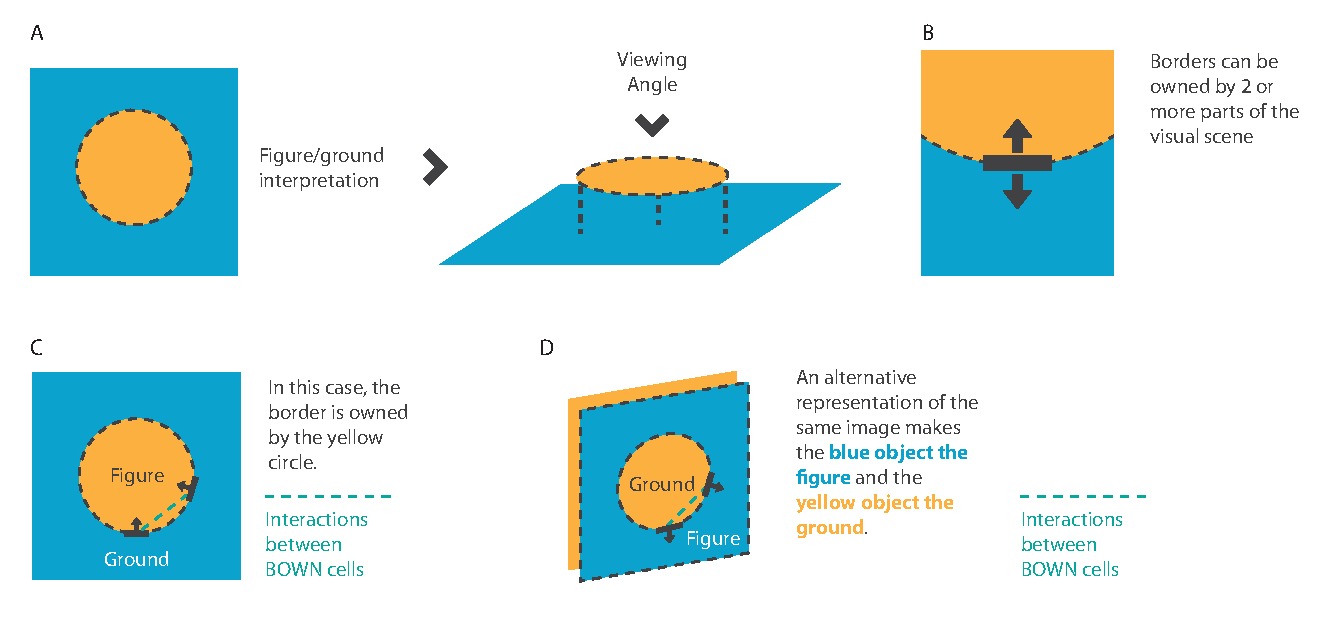
\includegraphics[width=\textwidth]{images/related-work/border-ownership}
\caption{A) This image is interpreted as an orange ellipse on top of a square.
B) A border can belong to two competing regions.
C) A competing side on a boundary becomes the owner which provides the relationship that the circle is the figure, and the rectangle is the ground.
D) An alternative representation of the same image shown in A) shows how depth can change the interpretation of the image.
Green lines illustrate Interactions between BOWN cells which are said to assist with creation of depth maps.}
\label{fig:bown}
\end{figure}

Border ownership appears to be facilitated by three types of neurons identified in V2 \cite{zhou2000coding, qiu2005figure} selective for \emph{side-of-figure} (35\%), \emph{depth order} (40\%) and both \emph{side-of-figure} and \emph{depth order} (21\%) \cite{qiu2005figure}. 
Neurons selective for side-of-figure have a preference for ownership at a particular side as shown in Figures \ref{fig:bown-examples} A and B. 
Figure \ref{fig:bown-examples} A shows how the BOWN neurons respond to a boundary only when it is part of a surface that lies on the preferred side of the cell's receptive field. 
In this case, the neuron is receptive to arrangements where the figure is on the right side. 
This is exemplified further in Figure \ref{fig:bown-examples} B with examples I)1 and II)1 where the spike rate of II)2 is ~4x that of I)1 when the figure is to the right of the receptive field. 
A similar result can be seen in the rest of the examples.  

\begin{figure}[t!]
\centering
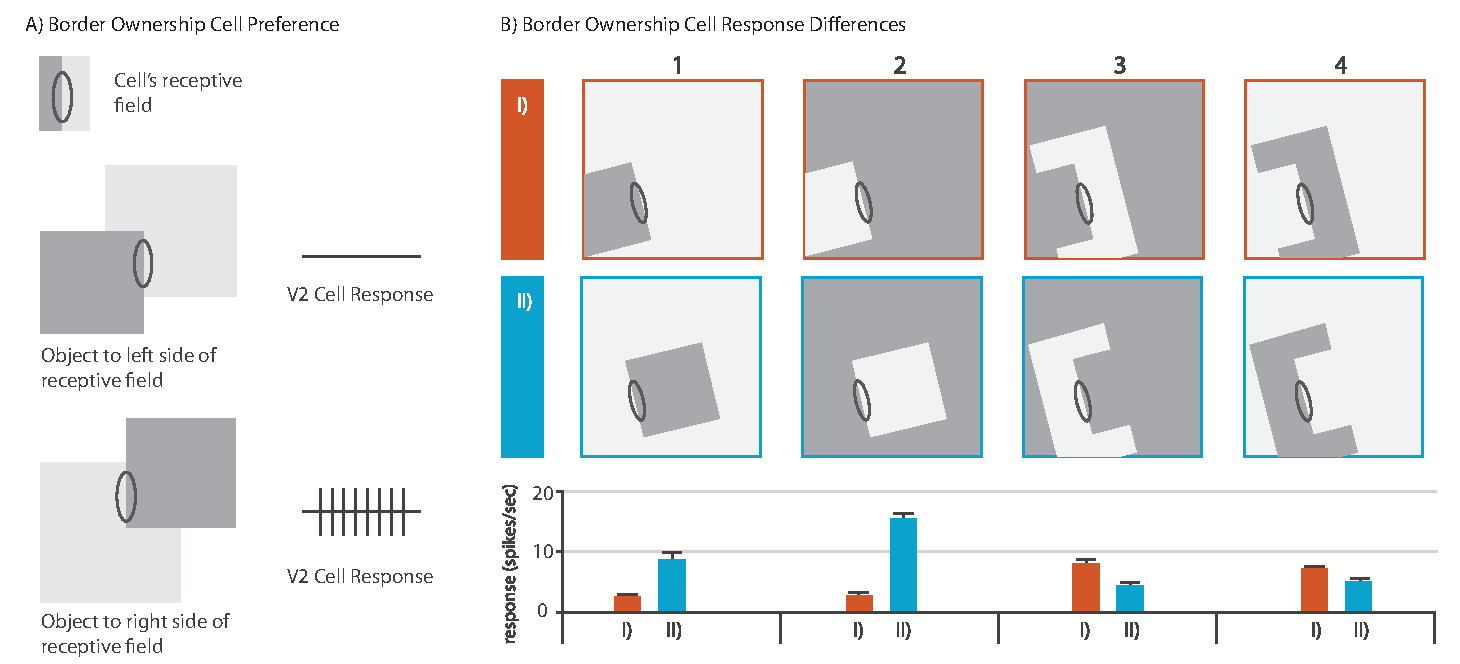
\includegraphics[width=\textwidth]{images/related-work/bown-neurons}
\caption{BOWN sensitive neurons with a preference for right-side figure in the macaque visual cortex. A) V2 cell response when object is on preferred side of a cell's receptive field (in this case, right). B) The oval with the black outline represents the receptive field which remains constant throughout all examples. Examples \textbf{I)} 1 and 2 on the top row (orange) show a number of examples of figure/ground scenarios with border ownership on the left side of the receptive field. The converse arrangement of \textbf{I)} 1 and 2 is shown on the bottom row (\textbf{II} 1 and 2). Examples \textbf{I} 3 and 4 show border ownership on the right side with left side ownership shown in \textbf{II} 3 and 4. Average neural responses are shown for each scenario (\textbf{I)} and \textbf{II)}). Modified from \cite{zhou2000coding, kandel2012principles}.}
\label{fig:bown-examples}
\end{figure}

Through point-wise border ownership calculations across all local contours of an object, with pairwise excitation of agreeing BOWN cells and inhibition of disagreeing BOWN cells, the visual system is able to discriminate between figure and ground and create depth maps.

\subsubsection{Motion Perception}
Analysis of motion is prevalent throughout the visual cortex from the retina \cite{kimspace2014, kandel2012principles} whose cells react as much to movement as to light (a static image would fade from view if it were not for the continuous movements of the eye, called \emph{saccades}) right through to the visual cortex. 
At different levels of the visual processing system, motion information is processed via direction-selective neurons. 
In fact, there are cells in the retina that only respond on the observation of local contours moving in particular directions. This has been shown in rabbits by Barlow \etal \cite{Barlow01021963} and more recently by Kim \etal \cite{kimspace2014}.
Kim \etal showed that such direction-specificity of neurons was present in the retina of mice through ``starburst neurons'' that operated via the process illustrated in Figure \ref{fig:motion-neurons}.
Such direction-specificity is made possible through time-delayed bipolar cells that must be activated in the correct sequence to illicit a response from the neuron \cite{kimspace2014}.

\begin{figure}[t!]
\centering
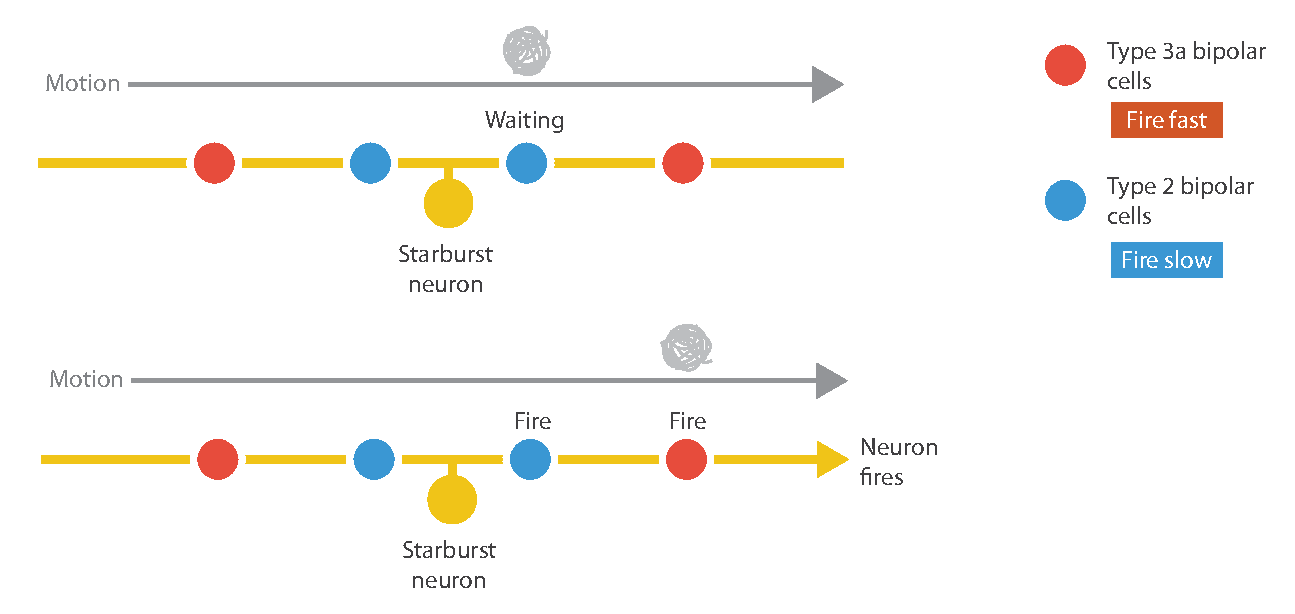
\includegraphics[width=\textwidth]{images/related-work/starburst-neurons}
\caption{Illustration of a starburst neuron (yellow) with two classes of bipolar cells to each side of the neuron. 
Type 3a bipolar cells (red) are farther from the cell body and fire immediately. 
Type 2 bipolars (blue) have a time delay and are close to the cell body.
When motion is detected, both types of cells issue a response, however the starburst neuron fires only when both cells have been activated in a specific order.
In the top image, a ball of string moves across the field of vision illiciting a response from a type 2 bipolar cell, which has a delayed response.
When the ball of string moves over the type 3a bipolar cell, a response is made immediately.
If the response from the type2, followed by the type 3a bipolar cell occurs at the same time, the neuron fires.
Modified from \url{http://blog.eyewire.org/eyewires-first-scientific-discovery-and-nature-paper/}}
\label{fig:motion-neurons}
\end{figure}

Movement is also processed in the visual cortex in both parvo and magno pathways.
These movement sensitive neurons can be classed as one of a number of types: 1) cells that respond to movement irrespective of form. This type can be subdivided in to: a) neurons that respond to motion in any direction; and b) those that respond to one direction; and 2) cells that respond to contour and movement together (almost all directionally selective) \cite{Zeki01021974}.
Similar to how neurons have distinct preferences for a particular orientation, neurons sensitive to motion have a preference for movements in particular directions \cite{maunsell1983functional, dubner1971response, krug2012principles}.
Additionally, these neurons also indicate the depth of the object in 3D space \cite{maunsell1983functional, dubner1971response, krug2012principles}.
As processing moves from the retina to V1, V2, then the middle-temporal (MT) area, there is an increase in the size of the receptive field. 
This represents a change in how processing moves from encoding local contour movement to global object movement.


\subsubsection{Analysis of Surface Properties, Depth and Segmentation}
Contour integration, object motion, and border ownership all contribute to the signals required to determine surface properties, depth, and segmentation. 
There are additional processing steps however using surface properties and depth to assist with object segmentation.

Surface properties (texture, colour, brightness) of an object are calculated through comparison of light arriving in different areas of the visual field. 
What is interesting about colour processing in particular is that even though the amount of available light can vary hugely throughout a typical day, our perception of object colour does not change much. 
This effect is termed ``perceptual constancy'' in the many examples provided by Beau Lotto\footnote{\url{http://www.lottolab.org/articles/illusionsoflight.asp}}. 
A possible explanation to this was given by Zeki who found neurons in V4 that elicit the same response to different illumination wavelengths if the perceived surface colour remains the same \cite{Zeki1983767}. 

Most of the neurons and receptive fields (retinal ganglion cells, LGN, and areas of visual cortex) are signalling contrast, and ultimately contours. 
Receptive field responses are low or non-existent for surfaces with no contrast. 
There are however a small number of neurons that respond to surface brightness, texture, and colour. 
These cells are heavily influenced through context provided by surrounding cells which may alter the perceived brightness. 
For example, in Figure \ref{fig:brightness-change} the brightness of an area surrounding a receptive field can result in perceived changes circle colour, where in fact there was none.
Due to an inequality in the number of neurons representing surface properties versus those dealing with contrast, there is a gap in visual information. 
To overcome this, the visual system performs what is called ``perceptual fill-in'' where the brightness of a surface is calculated from contrast information at the surface boundaries \cite{kandel2012principles}.

\begin{figure}[t!]
\centering

\includegraphics[width=.6\textwidth]{images/related-work/brightness-illusion}
\caption{The two circles are the same colour but the background affects perception with the one on the right appearing brighter due to the decreased brightness of the surrounding areas.}
\label{fig:brightness-change}
\end{figure}

\subsubsection{Depth Perception}
A further operation of this intermediate-level processing step is depth perception, made possible through a number of enablers. 
Information captured in the ocular dominance columns of V1 capture the binocular disparity (differences) created by the two versions of the world perceived by our eyes. 
From this information, a number of further processing tasks take place here to determine depth carried out first by a number of cells in the ocular dominance columns that are selective for objects at different distances.
These cells can be roughly categorised into three types: those with a preference for objects that are near; those with a preference for those that are far away \cite{kandel2012principles}; and those with a preference for objects on the plane of fixation (in between).

Determining depth is a global process that involves many cooperating cells. 
When there is uncertainty about the depth of an object in a group of cells, other cells with no ambiguity can feed information into those regions of uncertainty. 
This process is known as ``disparity capture''.
The global nature of disparity analysis is normally illustrated using random-dot stereograms \cite{julesz1971foundations}. 
These stereograms present what appears as noise to each eye, however when viewed binocularly (with both eyes), embedded shapes become visible\cite{kandel2012principles}.

\subsubsection{The Importance of Context}
The primary function of intermediate processing is to find objects in the scene by integrating the many constituent components of a visual scene. 
We are then able to take these objects and match them to its internal interpretation of previously encountered objects\cite{kandel2012principles}. 

This is not a one-way system and relies on an interconnected network of horizontal connections between cells at the same levels as well as feedback and feedforward system linking all levels of the visual system. 
This process of global integration can be facilitated through application of Gestalt laws about perceptual grouping along with additional high-level features such as attention, expectation, and past experience \cite{kandel2012principles}. 
This is referred to as a ``top-down approach'' and is discussed further in Section \ref{sec:topdown_bottomup}. 

\subsection{High-level Processing}

High-level processing refers both to the stage of visual processing where shapes and surfaces are identified, and in visually guided movement.
Here we focus directly on the former, in object recognition which relates specifically to the parvo pathway where processing continues from the visual cortex by passing surface and form objects to the temporal lobe for identification \cite{kandel2012principles}. 
However information about object movement from the magno pathway will also feed in to object recognition. 
Figure \ref{fig:high-level-processing} provides an overview of the tasks preceding high-level processing as well as the signals that help in object recognition. 
These signals involve:
\emph{working memory};
\emph{categorical linking};
\emph{associative linking};
\emph{signals from other senses} such as sound, smell, and touch;
and \emph{emotional valiance} which relates objects to past emotional events.

\begin{figure}[t!]
\centering
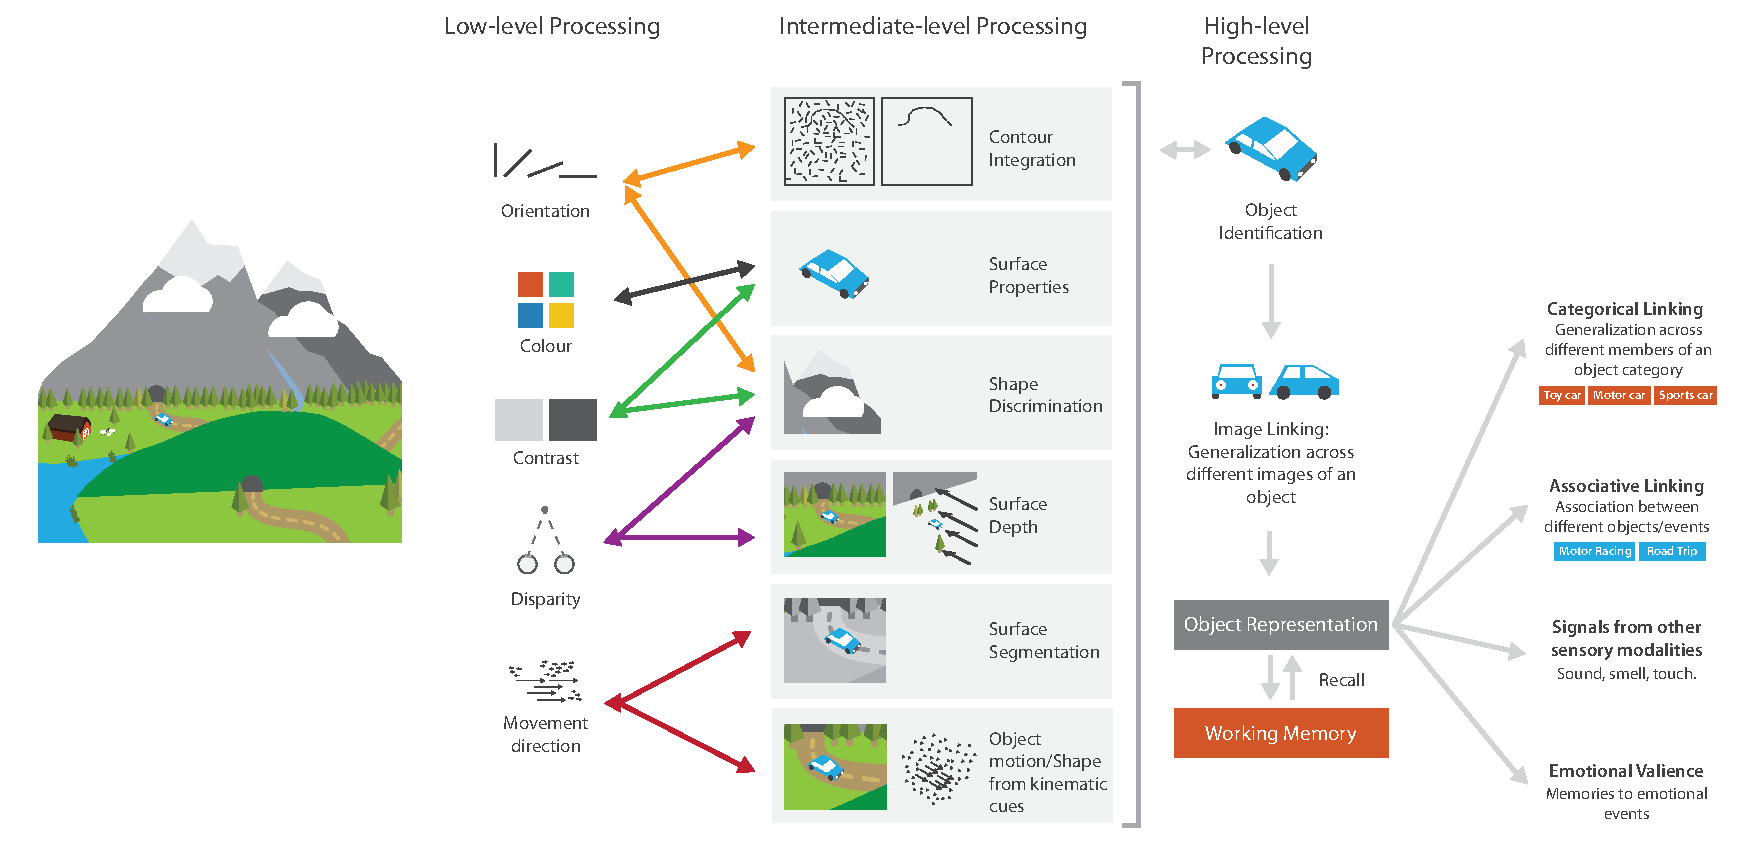
\includegraphics[width=\textwidth]{images/related-work/high-level-processing}
\caption{Flow of processing from low- to high-level processes with a focus on the object identification (parvo) pathway. Adapted from \cite{kandel2012principles}.}
\label{fig:high-level-processing}
\end{figure}

The brain's ability to identify objects is nothing short of amazing. 
Consider that the latest machine learning algorithms struggle to recognise different presentations of the same object. 
Brains on the other hand have been doing this for many thousands of years. 
There are a few areas of the brain responsible for this processing as illustrated in Figure \ref{fig:pathway-object-recognition}. 
The main part however is the inferior temporal cortex at the end of the ventral stream. 
This part of the brain has been clinically shown to be essential to object recognition \cite{kandel2012principles} via the introduction of lesions to this area of the brain in primates and observation of the consequences. 
When lesions were made in the inferior temporal cortex, an effect called \emph{visual agnosia} (coined by Sigmund Freud) was the result where the primates were unable to recognise objects \cite{kandel2012principles}. 
Later research observed this effect in humans and found that visual agnosia had two subclasses: 
\emph{apperceptive agnosia} where patients are unable to copy an object presented to them but they can identify the object \cite{Ferreira01091998}; and 
\emph{associative agnosia} where patients are able to copy the object but do not know what it is\cite{farah1990visual}. 
This research helped in further divisions of the inferior temporal cortex into posterior and anterior regions. 
The posterior region was associated with inability to see objects correctly and the anterior region was associated with assigning meaning to objects.

\begin{figure}[t!]
\centering
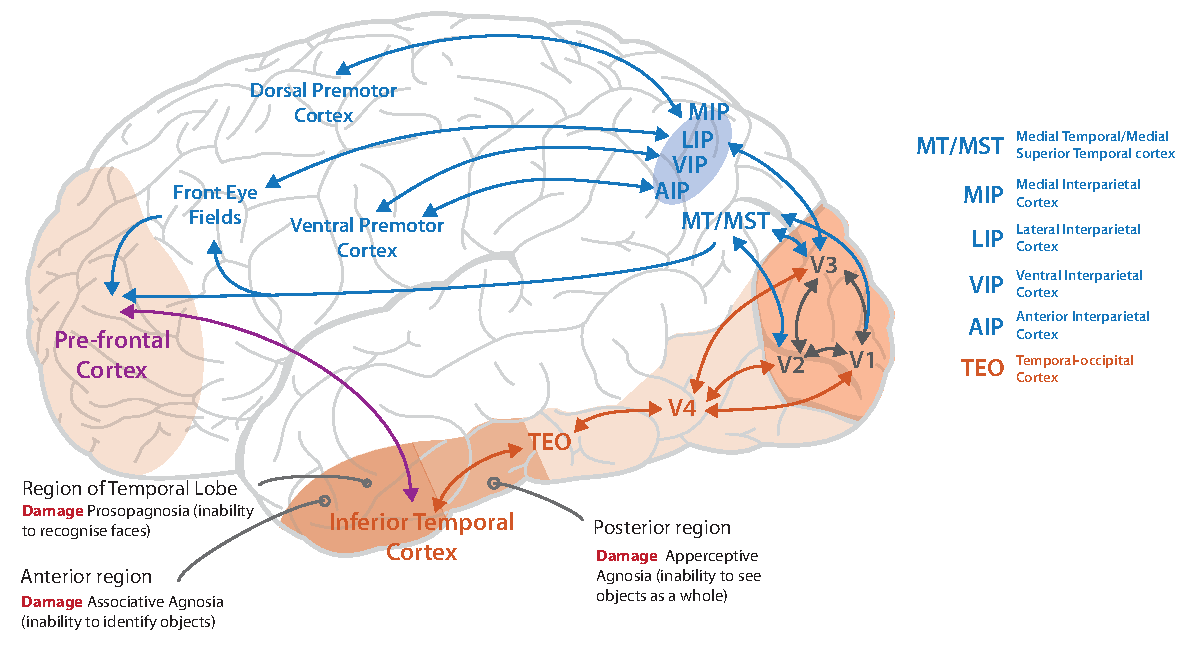
\includegraphics[width=\textwidth]{images/related-work/pathway-object-recognition}
\caption{Side view of the brain showing the object recognition pathway in orange. Adapted from \cite{kandel2012principles}.}
\label{fig:pathway-object-recognition}
\end{figure}

Similar to the early visual processing stages, neurons in the inferior temporal (IT) cortex have receptive fields that respond to distinct stimuli found using electrophysiological techniques. 
The IT is organised into columns with functional specificity to aid identification of particular patterns\cite{tanaka2003columns, kandel2012principles}. 
For example, some populations of neuron have been shown to be solely involved in face and hand detection in monkeys\cite{tsao2006cortical, tsao2008comparing, kandel2012principles}. 
Damage to these populations causes \emph{prosopagnosia} where the ability to recognise faces\cite{kandel2012principles} is lost. Face recognising cells are a population of cells with different preferences to the various ways in which a face may be viewed.
Some cells are shown to respond better to a frontal view of the face whereas others respond better to side profiles \cite{Afraz06, kandel2012principles}. 
These columns which identify different configurations of a face, pencil, computer or other complex forms are referred to as hyper-columns \cite{tanaka2003columns, kandel2012principles}. 
Due to the specificity of such hyper-columns to particular objects and shapes, it is reasonable to assume that the IT cortex is configured based on past experience. 
In other words, our past experiences influence the brain's ability to identify an object and will change in response to new information \cite{kandel2012principles}. 
Gilbert \etal call this process \emph{perceptual learning} \cite{Gilbert2001681}.

Aside from recognising the different configurations of an object in space, there are other problems left to be resolved in the visual system with respect to identifying an object similarly even though these objects may be far away or close by. 
Three populations of neurons have been shown to be involved in aiding a term previously introduced called \emph{perceptual constancy}, where objects can be identified even though they are different sizes (size constancy), have different positions on the visual field (position constancy) or have differences in reflectance (form-cue invariance) \cite{schwartz1983shape}. 

These properties of the object recognition workflow match those posed by Gestalt psychologists who cited \emph{invariance} as a key property of the visual system - the ability to identify items without the need for a precise match to what has been observed previously - referred to as the \emph{prototype} approach by Spoehr and Lehmkuhle \cite{spoehr82} and Franks and Bransford \cite{franks71}.

It should be noted that although a lot of information is known about the structure of the components in the high-level processes, little is known about how perceptual learning occurs, how objects are compared in the brain, how memories are formed, or how interaction between the IT cortex and long-term memory in the hippocampus works.

\subsection{Global and Local Processing}
\label{sec:global_local_processing}

A visual scene is arranged in a visual hierarchy \cite{palmer77, navon77, shor71, love99, kinchla79} where some pieces of information are more accessible than others. 
Large features in a scene such as a building, versus the smaller items that are less easy to see such as the writing on a poster placed on a wall will be more or less accessible to processing by our visual system depending on proximity. 
We will not be able to read the text on a poster for instance from 100 meters away but we will see the outline of the poster.
Global features such as overall shape, colour, \emph{etc.} will be accessible to the visual system from larger distances than local features such as the lines of text on a poster and the key factor is spatial frequency. 
The fovea, which represents the highest resolution are in the visual field has the smallest receptive field and therefore provides the greatest level of detail. Moving further away from the fovea the receptive fields become larger and the detail these areas capture becomes much more coarse \cite{kandel2012principles}.

\begin{figure}[h!]
\centering
\includegraphics[width=\textwidth]{images/related-work/spatial-frequency}
\caption{A) From further away, a letter will not be fully perceptible as a result of the receptive field in the retinal ganglion cells. 
A single letter could be represented by one receptive field which could be interpreted as nothing more than a blurry spot. 
When the letter is viewed up close, each of the local contours that make up the letter 'E' can be covered by individual receptive fields. 
B) Low detail image as would be seen by our visual system by large receptive fields. As we zoom into focus on particular areas, the granularity of the image keeps increasing until we have a fine-grained image. }
\label{fig:spatial-frequency}
\end{figure}

Figure \ref{fig:spatial-frequency} A serves to illustrate how local, or fine details like text or thin lines will not be readable from far away since the receptive field is not small enough to capture local contrast differences. 
Small text would appear as a blur. 
By decreasing the distance from the text, individual lines can be served by more receptive fields. 
The receptive fields provide the contour information used to encode the letter, and this information can then be passed on to higher levels to be further processed. 
Figure \ref{fig:spatial-frequency} B illustrates how global features such as overall shape, colour, and movement are more easily perceived at the overview level than low-level features such as the door outline on the barn. 
Objects such as the barn (red) pop out from the scene and demand our attention for example. 
Pre-attentive processing will be discussed in more detail in Section \ref{sec:popout}.


\subsection{Bottom-Up, Top-Down and Salient-Feature Detection}
\label{sec:topdown_bottomup}

Depending on what we are looking for, our system can be tuned to finding items very quickly whilst ignoring other items. 
If we are not looking for anything in particular, we may process a scene systematically to look for something interesting, or it could be that some items may be more prominent than others due to pop-out and will command our attention. 
A bright red stop sign in a road for example or the flashing lights of a police car. 
This set of possibilities for how we process a visual field can be classified as: 
\emph{bottom-up} where we start at the low-level features of a visualization and build up the entire image progressively\cite{marrvision}; 
\emph{top-down} where we see outlines of shapes, use context, and other high-level information to infer what those outlines correspond to, then look for the local features of those objects we expect to find \cite{lee2003computations}; and 
\emph{salient-feature detection} where items that pop out in a scene draw our attention and we process these items first. 

\begin{figure}[h!]
\centering
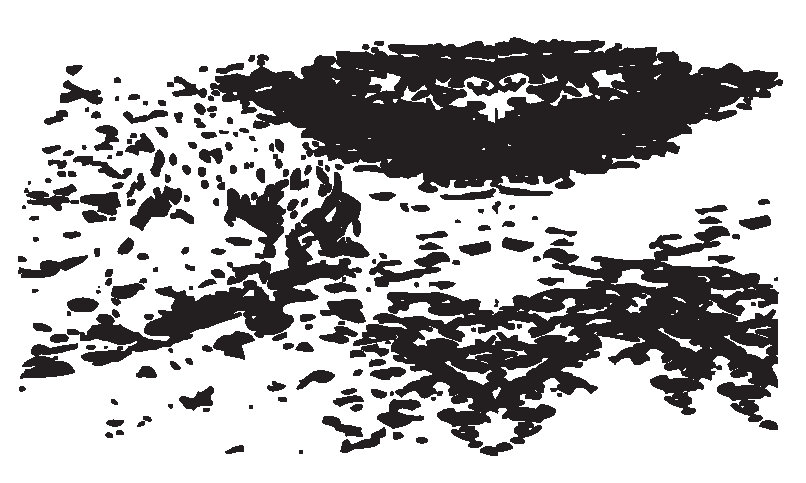
\includegraphics[scale=.55]{images/related-work/top-down-penguin.pdf}
\caption{This image depicts a Dalmation sniffing the ground and is an adaption of that produced by R.C. James and used by Lee \cite{lee2003computations}.
This example serves to show the power of top-down processing where knowledge of the dog in the scene helps in processing, whereas the use of local processing techniques leads to longer search times.
Before knowing a Dalmation is in the scene, viewers often struggle to see it.
This also illustrates a Gestalt effect with the dog shape being apparent even though parts of its body have not been explicitly defined.}
\label{fig:global-dalmation}
\end{figure}

Top-down and bottom-up processing are terms also used to describe the possible computational model the brain follows. 
Do the instructions for processing a scene come from the low-level features and progress through the visual cortex into the high-level object recognition phases (bottom up)? 
Or does it follow an approach where high-level information influences the sensitivity of particular neurons to particular colours, shapes, or textures (top down)? 
The general consensus is that it is not one or the other, but both. 
The visual system consists of a hyper-connected set of neurons with many feedback and feedforward systems enabling information from previous experience, context, and expectations to influence how a scene is processed by the visual processing components in the low- and intermediate- level processing stages of the visual system. 
Gestalt laws, in particular the idea of \emph{emergence} is illustrated in Figure \ref{fig:global-dalmation} where at first glance the subject of the image is unclear. 
For readers unaware of the subject, it could take a fairly large period of time to discover it - there would be a reliance on building the picture from the ``bottom up''. 
When told that the image represents a Dalmatian sniffing the ground, for many viewers, the outline of a Dalmatian will form as a result of our expectations of how a dog should look. 
These expectations tune the visual system to select for particular features (\eg, colours, contours, textures) that represent our inner ``template'' of a dog.
This is ``top-down'' processing.

\subsection{Pre-attentive Processing}
\label{sec:popout}

\begin{figure}[ht!]
\centering
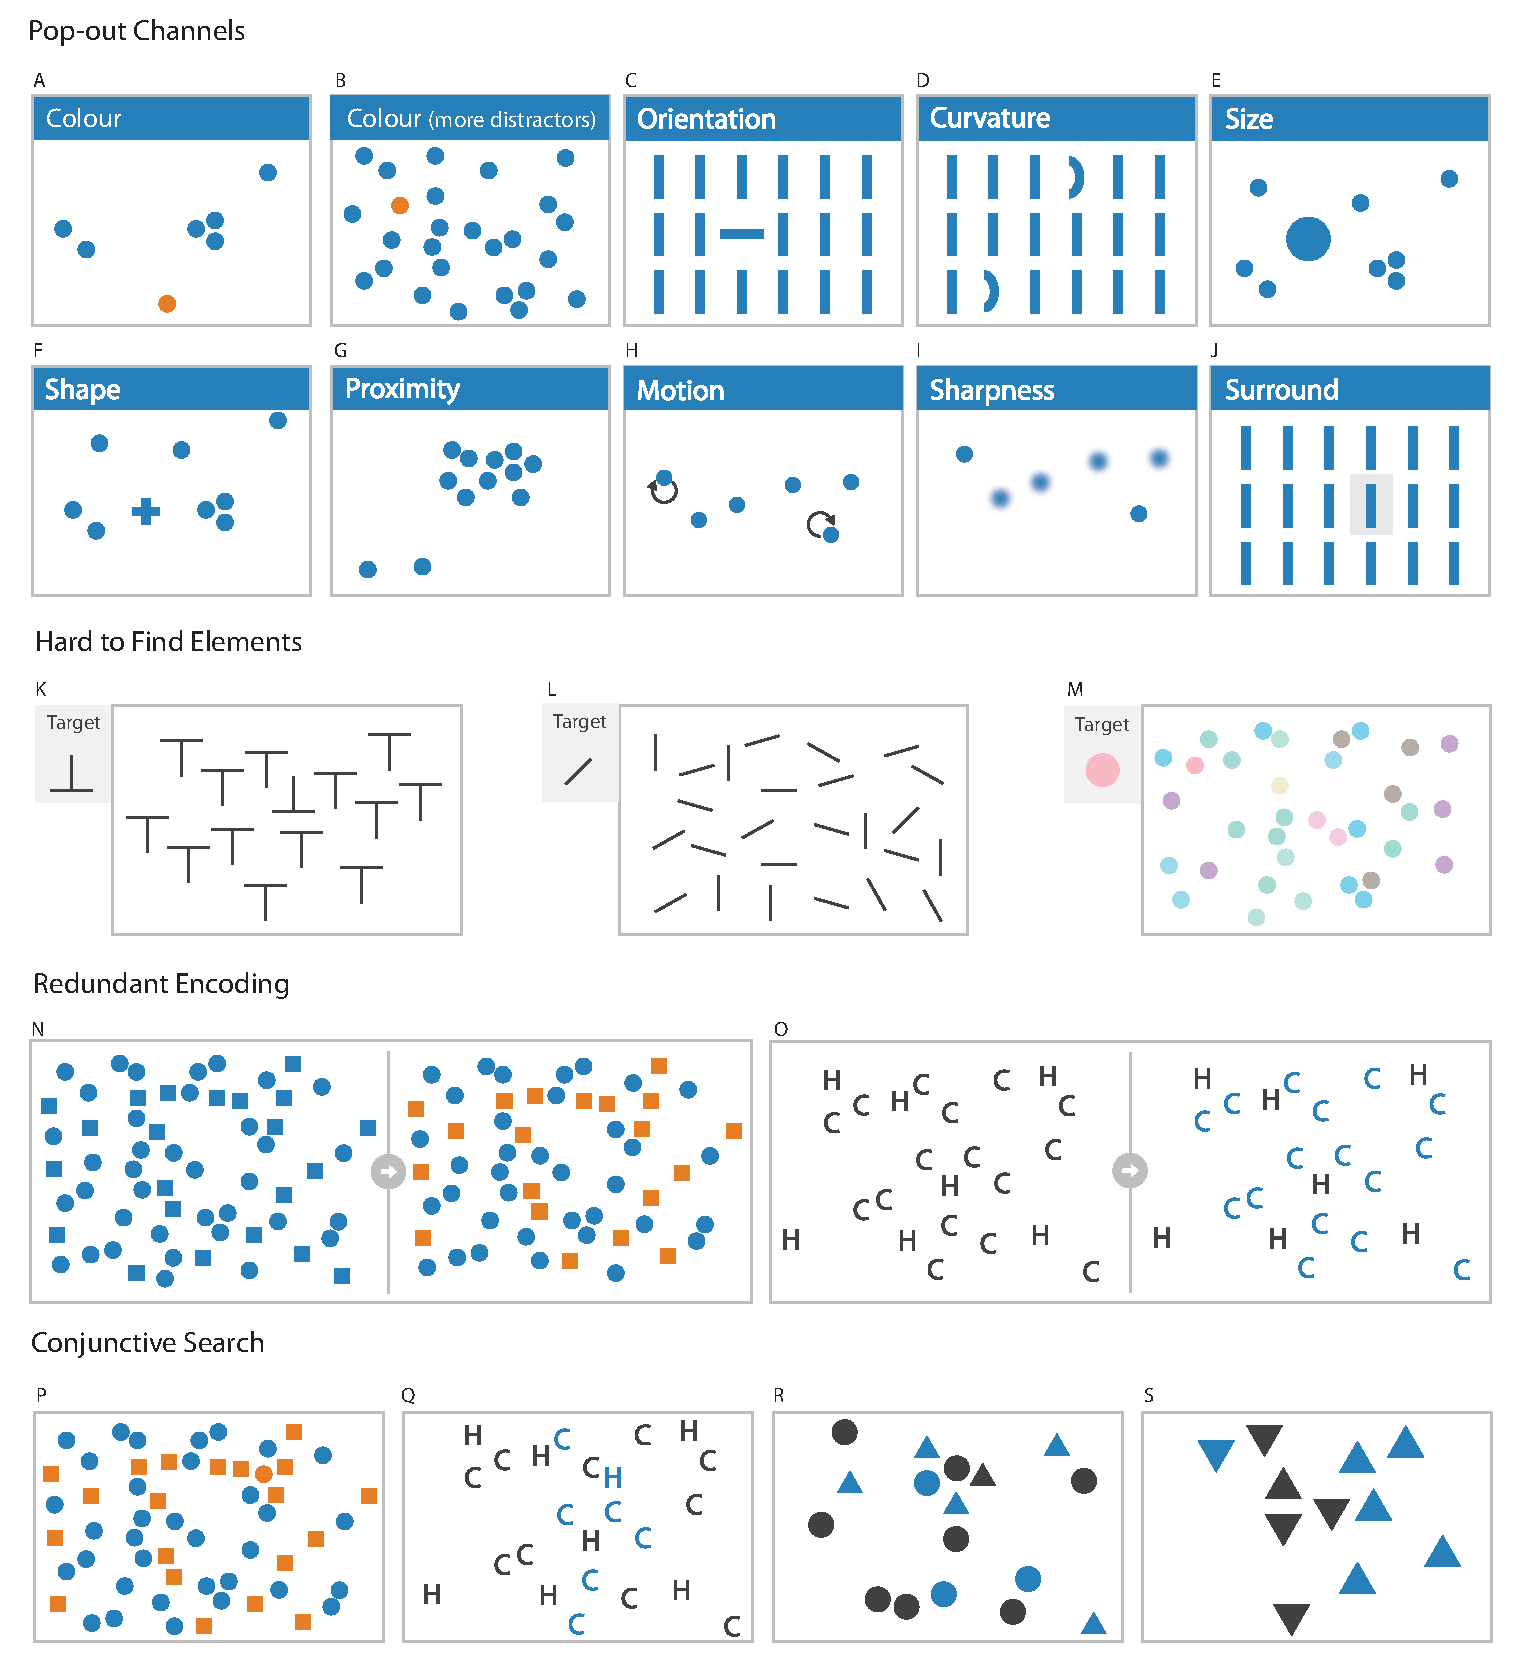
\includegraphics[width=\textwidth]{images/related-work/popout.pdf}
\caption{A to F) Visual channels amenable to pre-attentive processing. 
K to M) Examples illustrating where differences between the search target and distractors is not sufficient to enable fast visual search. 
N and O) The effect of redundant encoding on aiding visual search. 
P to S) Conjunctive search examples where in: 
P, the orange circle is the search target; 
Q, a blue H is the search target;  
R, a black triangle is the search target; and 
S) A upward pointing black arrow is the search target.}
\label{fig:popout}
\end{figure}

In 1988, Anne Treisman \cite{treisman88} first showed that the visual system was somehow able to tune visual attention to find particular objects with specific visual attributes \cite{kandel2012principles, treue1996attentional} in a very small period of time (less than 300 milliseconds).

From this research, a number of visual properties were identified that were shown to be processed by the low-level processing components of the visual system \cite{healey11}.
These properties came to be known as pre-attentive.
As a result of how pre-attentive visual properties visually stand out on a display, the effect is commonly and less formally referred to as the ``pop out effect''.

However the name pre-attentive is now misleading.
Research in 2002 by Kleinschmidt \etal \cite{kleinschmidt2002} showed how top-down feedback loops have been observed to play a role in pre-attentive processing by maintaining attention on a visual object.
This has been studied through observing a visual item gradually becoming visible amongst noise in a busy scene, then observing at what point the item no longer appears, termed ``drop-out''.
There is a difference in the points at which the visual item pops out and when it drops out \cite{kleinschmidt2002}. 
Kleinschmidt \etal found that drop-out occurred at a lower level than pop out occurred.
This effect is called \emph{hysterisis}.
Using fMRI with human participants, Kleinschmidt \etal \cite{kleinschmidt2002} were able to detect enhanced activity in the temporal, parietal, and frontal cortex that correlated with the preservation of the pop-out effect.
This study provides evidence of top-down processes being important in the pop-out phenomena.
Nevertheless, the term pre-attentive continues to be used to refer to visual items that can be found rapidly in a display \cite{healey11}. 


As shown in Figure \ref{fig:popout}, almost all visual channels support pre-attentive processing.
The speed at which these variables pop out however is not always the same.
The visual channels that perform best (derived from the psychology literature) can be ordered as colour $\prec$ size $\prec$ shape $\prec$ orientation (\eg, \cite{williams67,quinlan87,ropinski11}) where symbol $\prec$ reads as \emph{precedes}.
An interesting property of the pre-attentive processing is that it is not bound by the number of distractors in the scene\cite{ware13}.
In Figures \ref{fig:popout} A and B for example, the number of blue circles does not impact search on the red circle.

The effect of pre-attentive processing may be increased or decreased depending on how variables are combined with each other.
To increase, a technique called redundant encoding can be used where the visual representation of items in a display are encoded with two or more non-overlapping visual channels.
Figures \ref{fig:popout} N and O show this effect in action.
In Figure \ref{fig:popout} N, shape is used to solely distinguish two groups.
With the addition of colour in Figure \ref{fig:popout} O, the separation is more clear with one group represented with blue circles and the other with orange squares. 

To decrease or remove the ability to pre-attentively process a scene, one may reduce the visual distance, or noticeable difference between visual items in the display.
For example, in Figure \ref{fig:popout} B we have two hues with a large noticeable distance that lend themselves to fast visual search.
In Figure \ref{fig:popout} F we have seven colours within overlapping colour hues that have a much smaller noticeable difference between them.
In this example, visual search becomes more time consuming and erroneous.

Additionally, Figures \ref{fig:popout} C and L show the same effect for orientation.
In Figure \ref{fig:popout} C there are two orientations with a large difference.
Figure \ref{fig:popout} L shows an example with five orientations where finding the line with the correct orientation becomes very difficult.

Finally, by adding complexity to the search requirements, the speed of visual search will be further reduced.
In single feature detection, a participant in an experiment generally looks for a H amongst Cs. 
As found by Navon, this search environment lends itself to parallel processing so the distractors and targets can be processed simultaneously \cite{navon77}.
Where there are overlapping search criteria, this is termed ``conjunctive'' search which does not lend itself to parallel processing \cite{navon77}.
Take Figure \ref{fig:popout} Q where we search for a blue H amongst black and blue Cs and black Hs.
The visual system must first look for the blue items, which gives a mixture of Hs and Cs, then look for the Hs.
Due to the combination of features to be searched on, conjunctive search is generally slower than single feature detection \cite{quinlan87}.
This is a process illustrated in Figure \ref{fig:visual-search}.

\begin{figure}[t!]
\centering
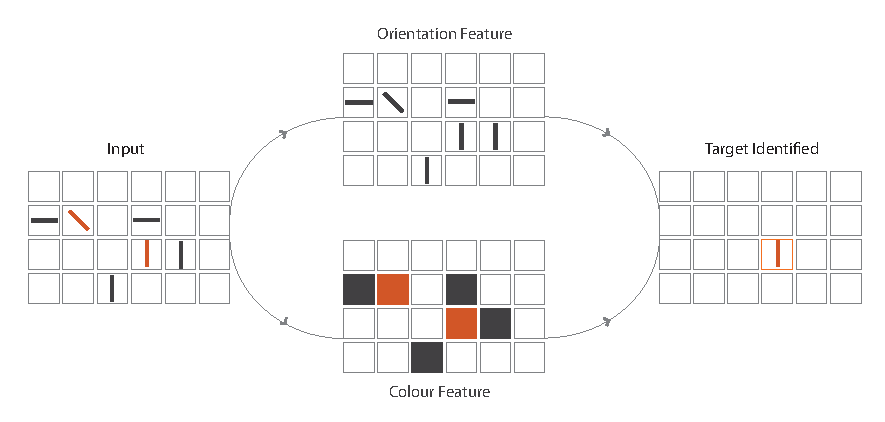
\includegraphics[width=.8\textwidth]{images/related-work/visual-search.pdf}
\caption{An illustration of how feature detection is said to work. This process is often posed as either a parallel or serial function and shows how in a visual scene of orange and grey lines how one may pick out the vertical orange line through combining the results of the orientation and colour feature searches together.} 
\label{fig:visual-search}
\end{figure}

The neurophysiological explanation for why visual elements in a display are available of pre-attentive processing or ``pop out'' is largely cited as being caused by contrast differences, and a top-down feedback loop that maintains attention on the concept that has popped out.
Contrast differences have been shown in centre-surround cells in V1 that select for orientation by Schmid and Victor \cite{Schmid2014}, illustrated in Figure \ref{fig:orientation_rf}.

\begin{figure}[t!]
\centering
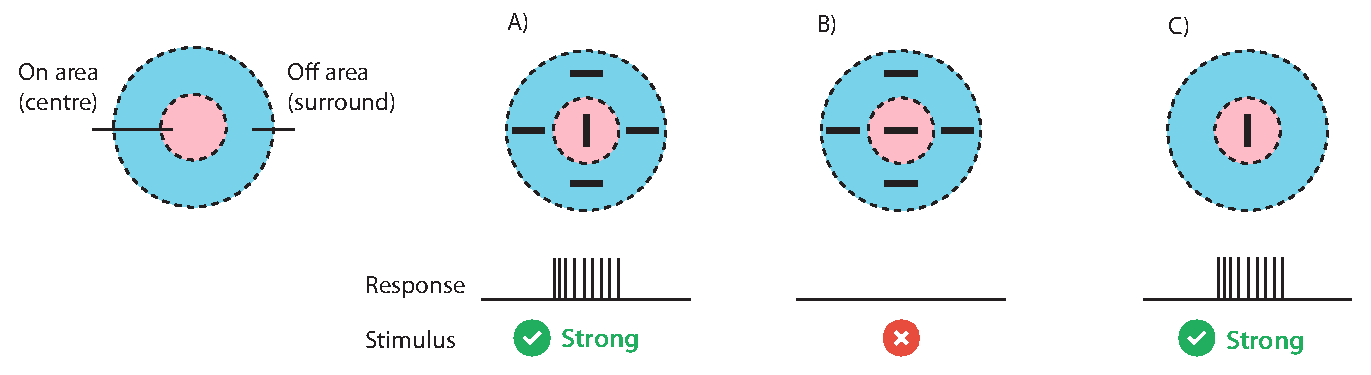
\includegraphics[width=\textwidth]{images/related-work/orientation_rf.pdf}
\caption{Based on those reported by Schmid and Victor \cite{Schmid2014}. A) With the orientation in the centre different from the surround, a strong response is recorded from the cell.
B) When orientation is the same in the centre and surround, no response is output. C) With an orientation detected in the centre but not in the surround, a strong response is output.} 
\label{fig:orientation_rf}
\end{figure}

When the orientation in the centre of the receptive field differs from that in the surround, the neuron response is high (Figure \ref{fig:orientation_rf} A).
If the orientations are the same, there is no response (Figure \ref{fig:orientation_rf} B and C).
Further studies would be needed to confirm similar receptive fields for colour and position for example, and at the higher levels of the visual processing pipeline, such as in V4 which deals with more complex forms.


\subsection{Integral and Separable Dimensions}
\label{sec:channel-composition}

 \begin{figure}[t!]
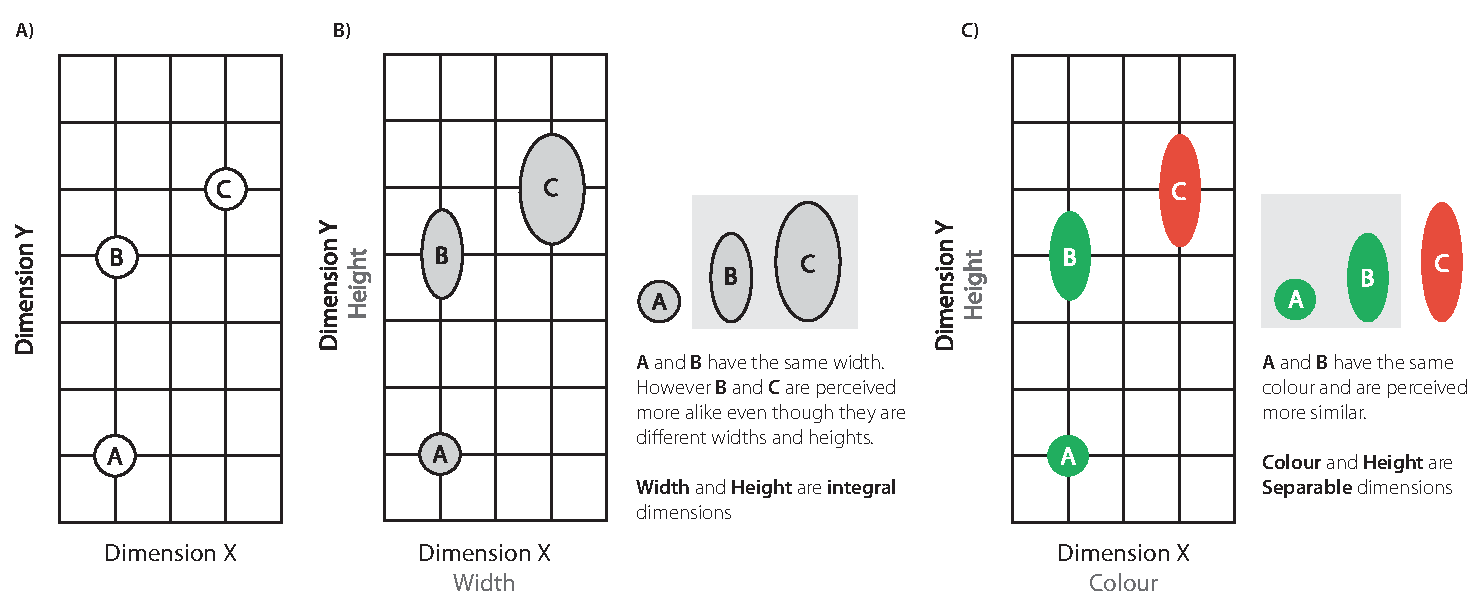
\includegraphics[width=\textwidth]{images/related-work/integral_separable}
\caption{Some examples from Ware \cite{ware13} to explain integral and separable dimensions. A) Ware \cite{ware13} used this grid to help designers think about separability of dimensions. B) Replacing dimensions X and Y with width and height respectively, we can see that even though A and B have the same width, B and C are perceived more similar. These dimensions are integral. C) With colour replacing width, A and B are now perceived more similar, which is the desired effect. These dimensions are separable}
\label{fig:integral_separable}
\end{figure}

The theory of integral and separable dimensions was developed by Garner \cite{garner1974processing} in his book \emph{The processing of information and structure} based on a number of experiments by Attneave\cite{attneave1950dimensions}, Garner and Felfoldy \cite{garner1970integrality}, and Shepard \cite{shepard64}.

\emph{Integral} dimensions are perceived together instead of independently. 
As an example, Figure \ref{fig:integral_separable} B shows some simple glyphs as an ellipse whose width is mapped to dimension X and height is mapped to dimension Y of some data record. 
Even though glyphs A and B are more similar with the same width, it is B and C that are visually more similar. 
The overall shape of the ellipse is perceived rather than its individual parts (width and height).  
Previous research by Attneave \cite{attneave1950dimensions}, Shepard \cite{shepard64}, Krantz and Tversky \cite{krantz75}, and Handelt and Imai \cite{handelt72} found that integral dimensions exhibit what is known as a Euclidean distance (shortest path) defined as $\sqrt{d^2_a + d^2_b}$.
This has been recently validated by Demiralp \etal \cite{demiralplearning} in a large crowd sourced experiment.

\emph{Separable} dimensions are perceived independently.
This means, that converse to the integral dimension example, the individual components of the glyph can be perceived. 
In Figure \ref{fig:integral_separable} C, an ellipse glyph has its colour mapped to dimension X and height mapped to dimension Y. 
This has the effect of making glyphs with the same value of dimension X more similar, and can therefore be selected from the visual scene more easily.
Separable dimensions exhibit a city-block distance where distance is defined as $d_a  + d_b$ \cite{burns78,shepard64}.
This has also been recently validated by Demiralp \etal \cite{demiralplearning}.


What is important to note here is that defining a pair of visual channels as integral and separable is not always a binary classification. 
Both classes are on a continuum as shown in \ref{fig:integral_separable_continuum} where some pairs, such as width and height are fully integral pairs, whereas group location and colour are fully separable pairs. 
Additionally, as Ware states, the theory is very simplistic, and has many exceptions to the rule \cite{ware13}.
However, it does have merits as a design principle and can help designers avoid well-observed problems with the use of particular combinations of visual channels to encode data attributes.

 \begin{figure}[t!]
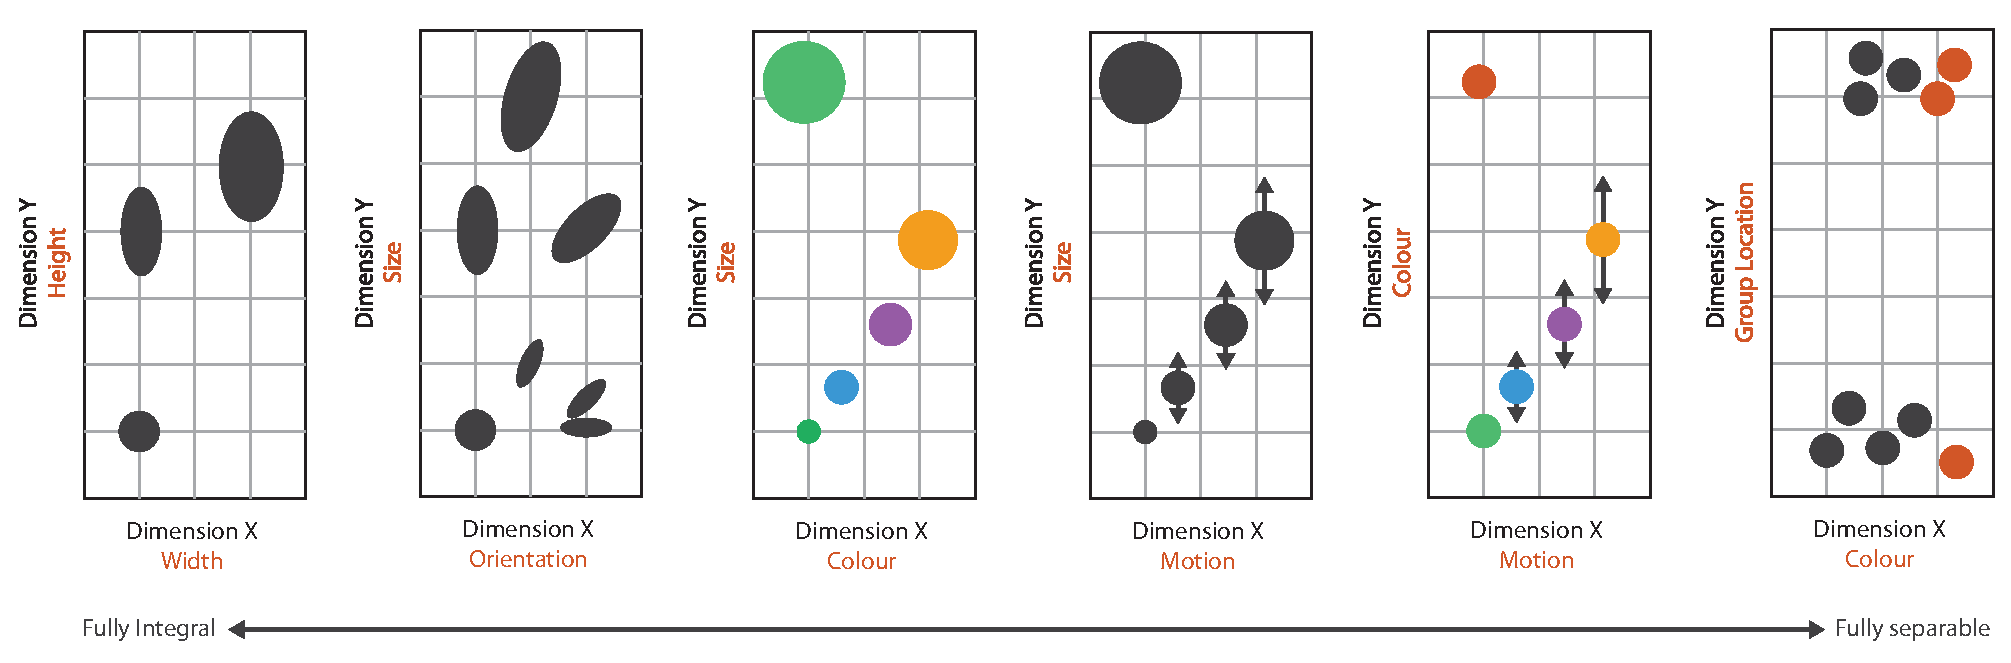
\includegraphics[width=\textwidth]{images/related-work/integral_separable_continuum}
\caption{Adapted from examples by Ware \cite{ware13} to show how pairs of dimensions may not by fully separable nor fully integral, but somewhere on a continuum.}
\label{fig:integral_separable_continuum}
\end{figure}

A full neurophysiological explanation for channel composition is not fully known.
However, a possible explanation lies in how the populations of neurons that process features may have an effect on integrality and separability of the channels they encode.
For example, Garner found that orientation is perceived independently of colour \cite{garner2014}, and Hubel, Wiesel and Livingstone found that shape and orientation are encoded by separate neural populations \cite{hubel1968, livingstone1988}.
Conversely, as stated by Garner \cite{garner2014}, Ganel \etal \cite{ganel2006}, and Drucker \etal \cite{drucker2009}, integral dimensions such as width and height are encoded by overlapping neural populations.

As previously stated by Kandel \etal, the size of the receptive field grows as one progresses through the visual system \cite{kandel2012principles}.
Features coded by overlapping neural populations (such as width and height) are likely to be merged later in the visual processing step and perceived and stored in working memory as an integrated object.
On the other hand, features coded by distinct neural populations will not be merged in to one, and will be stored in working memory as separable objects, and so will be perceived independently.

\subsection{Summary}
In this section we presented the building blocks of a visualization (visual channels), their power in representing particular types of data, and how these visual channels are processed by the visual system.
Additionally, we have discussed concepts of particular importance in glyph design including global and local processing, how feedback between multiple parts of the visual system can affect perception (bottom-up, top-down, and salient feature detection), pre-attentive processing, Gestalt effects, and integral/separable dimensions.

The goal of this section is to bring attention to what is already known from the cognitive sciences and attempt to explain why these effects happen.
Moreover, we aim to use the information presented here to guide users in the design of glyphs.



\section{Glyphs and Glyph-Based Visualizations}
\label{sec:relwork_glyphs}
The word \emph{glyph} is derived from the Greek word \emph{glyph$\bar{e}$} which means carving.
From the Palaeolithic age (18,000 BC) and their use of cave paintings, to the Neolithic age with petroglyphs (``stone carving''), pictures have been used to tell a story using symbols to depict particular events, objects, places, and activities (pictograms) or ideas (ideograms).
What is interesting about such pictorial approaches to story telling and communication is that there is a great intersection between visual language across vast different geological areas \cite{Eliade1991}.
This finding would indicate that symbols are key to the human conceptual system and that many of these symbolic representations are ``hard-wired'' in the brain \cite{Borgo:2013:EG,Eliade1991}.
Additionally, Egyptian hieroglyphs involve a more complex set of glyphs that pictorially represented not just ideas (ideograms), but also phonetics, and morphemes (the smallest grammatical unit of language).
The Chinese language with approximately thirteen dialects looked to pictograms and ideograms to solve communication problems between populations from different areas.
Perhaps the pictorial representations are not so clear in modern Chinese, however as illustrated in Figure \ref{fig:chinese-evolution}, this visual language has evolved from very metaphoric representations to their more abstract representations used today.
An additional feature of the Chinese language is how glyphs can be combined logically to mean something new, \eg, \emph{human being} can be combined with \emph{two} to mean \emph{humane}. 

\begin{figure}[b!]
\centering
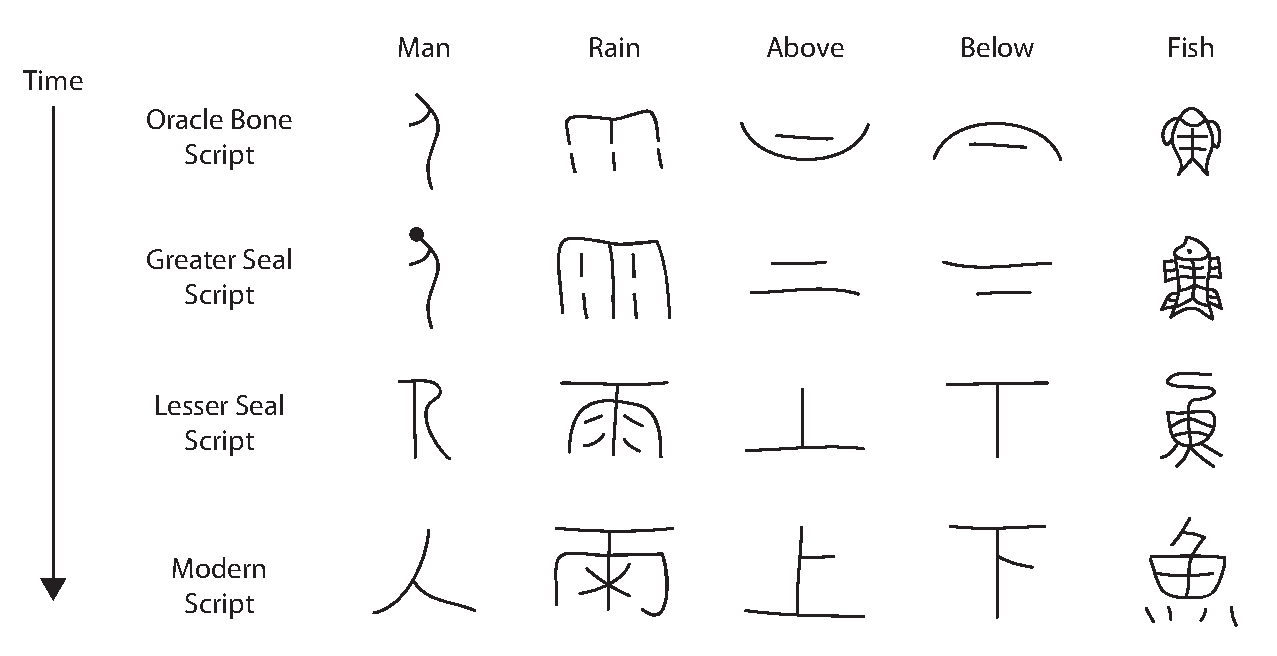
\includegraphics[width=.7\textwidth]{images/related-work/glyphs/chinese-pictograms}
\caption{The evolution of pictorial representations adapted from \url{http://www.ocf.berkeley.edu/\~wwu/chinese/handout.html} show how pictograms have evolved into more abstract representations over time with the use of different script styles.}
\label{fig:chinese-evolution}
\end{figure}

These examples show that glyphs are not a new concept, they have been used for many thousands of years to communicate across cultures and languages.
Even now they are used in language and are prevalent in human-computer interaction via metaphoric icons representing functions. 
The definition of glyphs by Borgo \etal \cite{Borgo:2013:EG} as \emph{small visual} objects that have a \emph{meaning}, involve \emph{learning}, and are often \emph{metaphoric} bridges the definitions of glyphs in ancient Chinese writing, Hieroglyphs, and Petroglyphs to the definition of glyphs used in visualization.
The primary difference is in that instead of solely representing ideas or physical objects, glyphs for multivariate data exploration depict qualitative and/or quantitive attributes of data records using combinations of visual channels \cite{Borgo:2013:EG}.
The result should be a \emph{small, visual} object that encodes multiple dimensions (has \emph{meaning}), and requires some \emph{learning} like those glyphs shown in Figures \ref{fig:glyphs-simple-complex} A and B.
Figure \ref{fig:glyphs-simple-complex} A shows a relatively simple glyph design encompassing five dimensions: wind speed, wind direction, temperature, and location (X and Y position).
The use of metaphor, in colour for temperature, arrow orientation for direction, proximity for speed, and position for location makes this glyph intuitive to decode. 

A more complex example is given in Figure \ref{fig:glyphs-simple-complex} B) created by Duffy \etal \cite{Duffy:2014:TVCG} who encode twenty-three data attributes in a single glyph.
The overall objective of this work is the creation of a summary visualization to reduce the need for domain experts to watch and re-watch videos.
Each glyph is used to summarise one second intervals of sperm video data.
These sperm glyphs are viewed with respect to their spatial setting with each glyph representing one second of activity for each sperm cell.
Domain experts can easily get an overview of the movement of the cell and its detailed properties through one image.

Both examples have illustrated the special ability of glyph-based visualization to preserve spatial information that would not be possible using parallel coordinate plots or scatter plot matrices.
Glyph placement strategies have been covered in detail by Matt Ward's \cite{ward02} excellent survey.
This work provides a comprehensive taxonomy of different layout algorithms in 2D or 3D space: data-driven (raw); data-driven (derived); and structure-driven.

\begin{figure}[t!]
\centering
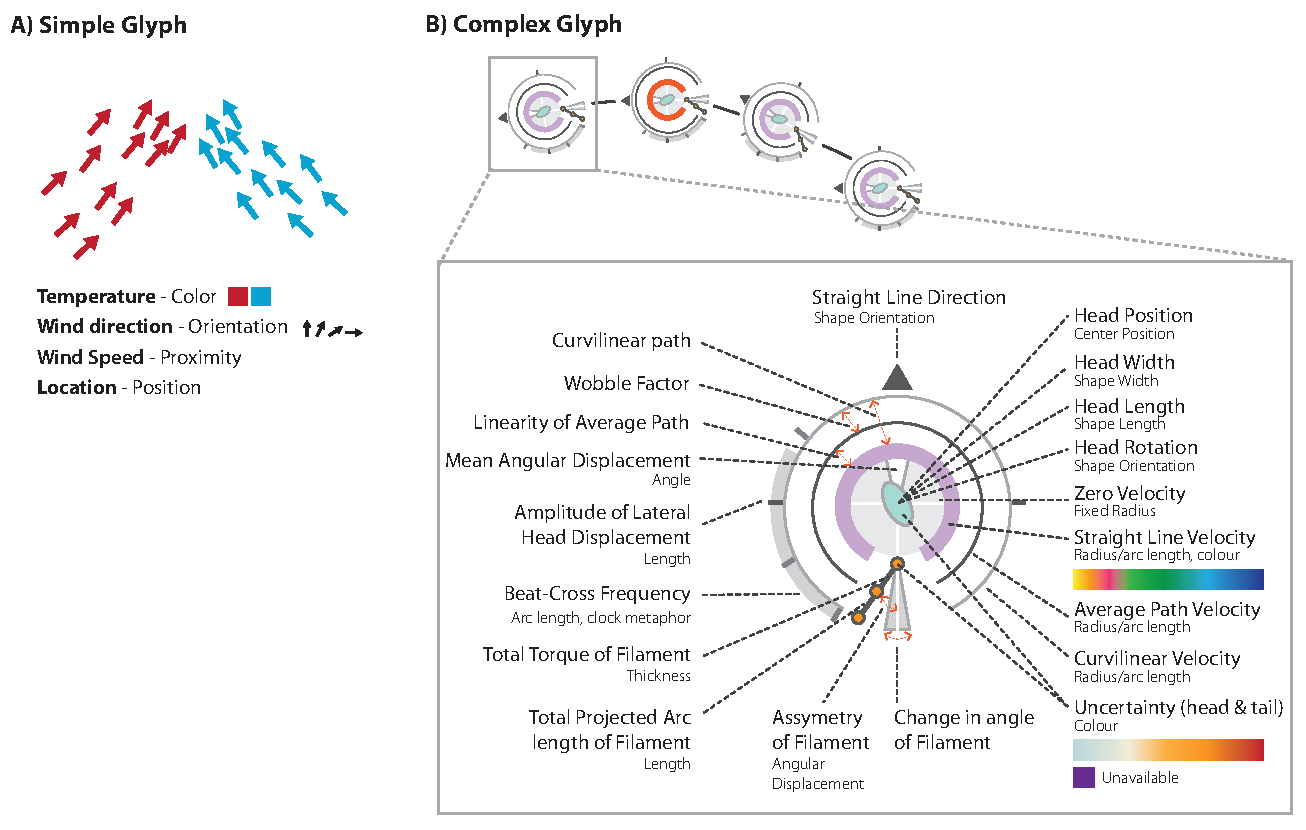
\includegraphics[width=\textwidth]{images/related-work/glyphs/glyph-simple-complex}
\caption{A) A relatively simple glyph for display of weather with five dimensions: wind speed, wind direction, temperature, and location (X and Y position). B) A more complex glyph with twenty-three dimensions by Duffy \etal depicting the attributes of sperm cells \cite{Duffy:2014:TVCG}.}
\label{fig:glyphs-simple-complex}
\end{figure}

These examples illustrate the power of glyphs in three ways: \textbf{1) multi-dimensionality} - glyphs can represent a large number of dimensions; \textbf{2) compactness} - they are able to ``compress'' a large amount of information in to a small space; and
\textbf{3) spatial preservation} - the ability to keep spatial information whilst overlaying more information.


\subsection{Glyphs and their Visual Encoding}
\label{sec:mapping-glyph-data}

Creating a glyph is often more involved than randomly assigning a data attribute to shape, colour, texture, size, or orientation.
Similar to visual signs or fonts, the design of a glyph set is in essence a visual coding scheme \cite{Borgo:2013:EG}.
Like all coding schemes, a well-designed glyph-based visualization can facilitate efficient and effective information encoding and visual communication \cite{Borgo:2013:EG}. 
A bad glyph design on the other hand may lead to ambiguity and confusion. 
Examples of good and bad coding schemes are shown in Figures \ref{fig:signs-code} A, B and C with examples based on letter discrimination and road sign design. 

Figure \ref{fig:signs-code} A shows how font choice, in essence a coding scheme, is important in the interpretation of letters. 
Using the \emph{Myriad Pro} font, many letters will not be ambiguous, such as \emph{a}, \emph{b}, and \emph{c}, however some letters will introduce ambiguity.
In the case of Illinois, the uppercase \emph{i} is not distinguishable from the lower case \emph{L}. 
While this ambiguity can be removed via context and past experience (\eg, knowing how to spell Illinois), it is a problem when previous context is not available, as is the case when learning another language. 
Change the font to \emph{Courier New}, and the ambiguity has been removed. 
Similar difficulties may arise when comparing \emph{\emph{S} and \emph{5}}, \emph{\emph{B} and \emph{8}}, \emph{\emph{A} and \emph{4}} for instance.

\begin{figure}[t!]
\centering
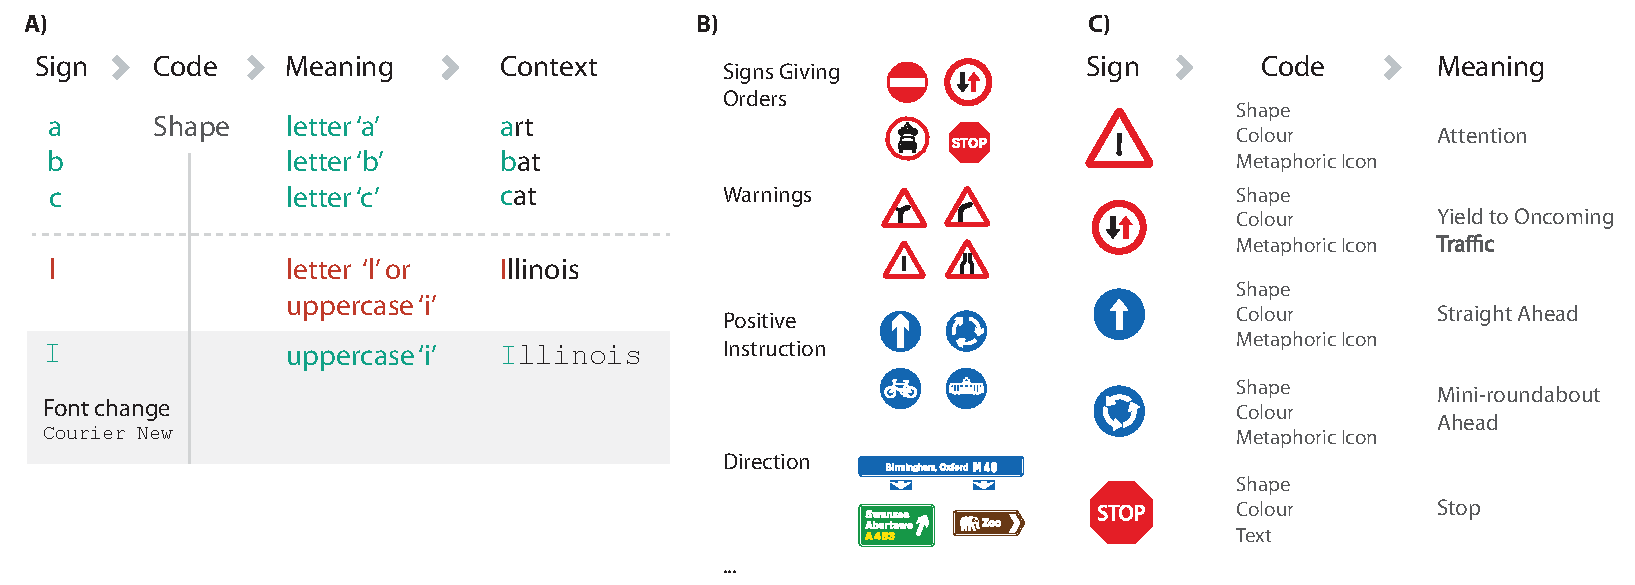
\includegraphics[width=\textwidth]{images/related-work/glyphs/signs-codes}
\caption{A) Letters are simply shapes that we assign meaning to. 
The code for creating such a shape is a particular font. 
With certain fonts, the differences between the letters is not sufficient, making it hard to find the meaning of a particular code. 
In this example, an uppercase \emph{i} can be confused with an \emph{l} (lower case \emph{L}) using the \emph{Myriad Pro} font, but is communicated more clearly using a font such as \emph{Courier New}. 
B) Road signs of the United Kingdom share some clear characteristics in different categories to make it more easy for drivers to visually select for particular pieces of information. 
C) Each sign is encoded with some information, normally pictorially to aid use by visitors from other countries and to encourage adoption as a standard across countries.}
\label{fig:signs-code}
\end{figure}

Figure \ref{fig:signs-code} B presents some classes of road signs for the United Kingdom. 
Road signs have been used for many years and have been iterated on heavily since the late 1950s \cite{kinneir1980words}. 
These iterations were made to ensure that drivers are able to find the information they are looking for (directions, warnings, \emph{etc.}) and that the most important messages are immediately visible to drivers (\eg, warnings and orders). 
If all road signs had the same general design, it would be difficult for drivers to select those signs that are important for safety from those that merely indicate the next service stop. 
If every road sign was too different from the next, drivers would have too much to remember. 
Designed by Kinneir and Calvert, U.K. road signs presented a solution in the form of categories of signs related to the type of message being communicated. 
These road signs had the additional requirement of being universally interpretable which brought challenges in ensuring visitors from other countries could recognise the signs and learn them quickly. 
This is similar to the requirement of the Chinese language to be readable by speakers of all thirteen dialects. 
This was enabled through adoption of European road signage protocols where circles indicated \emph{orders}, triangles indicated \emph{warnings}, and rectangles indicate \emph{information}. 
Colour was used carefully to add further discriminability (termed as \emph{redundant encoding}) to classes of signs, \eg, red for important warnings or orders, and blue for information signage. 
Finally, heavy use of text in previous road signs made it difficult for drivers from other countries to understand. 
Calvert introduced the use of pictograms instead of text where possible to refer to services, museums, men at work, and so on. 
This collective use of categories, shape, colour, and pictograms gave rise to the highway code, a visual language for the road in place since 1958 and a fine example of good glyph design.

Figure \ref{fig:signs-code} C illustrates a \emph{sign - code - meaning} relationship for road signs. 
In these examples and those in Figure \ref{fig:signs-code} B one may see that shape and colour play a large role in determining the type of sign while metaphor is used as much as possible to provide the internal shape. 
Metaphor is very important in the creation of signage due to the lower overhead required to remember what a sign means. 
Too many abstract shapes and colours would place a large cognitive load on anyone trying to decipher one of these codes. 
Additionally, important road signs such as \emph{stop} and \emph{no entry} are different from other signs under the \emph{giving orders} category due to their importance on the road. 
Not stopping at a junction or going up a one way street have the potential to cause great damage. 
Therefore these signs have a full red background which has a metaphoric relationship with \emph{danger}, with white text/shapes in the middle. 

\subsection{Glyph-based Visualizations}
\label{sec:glyph-examples}
From Chernoff faces \cite{chernoff1973use}, a generic glyph technique using facial attributes to represent data, to more application-specific glyphs such as the sperm glyphs by Duffy \etal \cite{Duffy:2014:TVCG}, glyphs have been used as a visualization technique across many diverse areas. 
Matt Ward provided an excellent summary of different types of glyphs in his 2002 paper \cite{ward02}.
The glyphs he identified, summarised in Figure \ref{fig:wardglyphs} included: profile glyphs (using height and colour of bars); star glyphs; Anderson/metroglyphs; stick figures; trees; auto glyphs; boxes; hedgehogs; Chernoff faces; arrows; polygons; dash tubes; weathervanes; circular profiles; colour glyphs; bugs \cite{chuah1998}; and wheels \cite{chuah1998};.

\begin{figure}[h!]
\centering
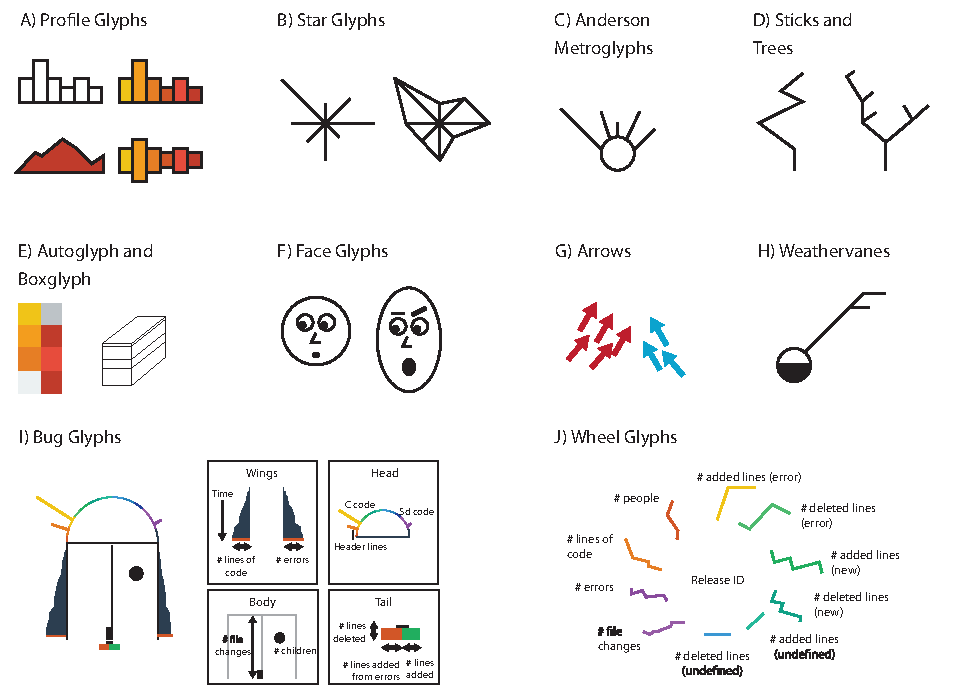
\includegraphics[width=\textwidth]{images/related-work/glyphs/glyphs_ward}
\caption{Some glyph examples from Ward \cite{ward02} with A) variations on profile glyphs; B) star glyphs; C) metroglyphs; D) stick and tree glyphs; E) Autoglyph and box glyphs: F) face glyphs (Chernoff faces); G) arrow glyphs; H) weathervanes; I) bug glyphs; and J) wheel glyphs.}
\label{fig:wardglyphs}
\end{figure}
 
Additionally, here we summarise the contribution glyphs have made in medical, event, geo-spatial, software management ,and search result visualizations.

\textbf{Medical visualization} has benefited from glyph-based visualization. 
They have been used for:
cardiac data by Ropinski and Preim \cite{ropinski08,ropinski11}, Oeltze \etal \cite{oeltze2008glyph}, and Meyer-Spradow \etal \cite{meyer2008glyph};
brain imaging, specifically (functional) magnetic resonance imaging ((f)MRI) by Tory \etal\cite{tory2001visualization}, Westin \etal \cite{westin02processing}, Zhukov and Barr \cite{zhukov2003heart}, Kindlmann \cite{kindlmann2004superquadric}, and Basu \etal \cite{basu2006rician};
and computerised tomography (CT) by Ropinski \etal \cite{ropinski2007surface}. 
A typical use case for glyphs, as identified by Ropinski and Preim, is where data from multiple sources (CT, positron emission tomography (PET) and MRI) are combined \cite{ropinski08}. 
MRI and CT data provide a detailed, high-resolution view of the anatomical structure whereas PET scans show cells that are metabolically highly active with the inclusion of glucose in the PET tracer along with a radioactive label. 
Tumour cells are typically more metabolically active than normal cells; therefore their need for energy, and therefore glucose is increased.
PET scans show these areas of activity and are pointers towards cancer sites. 
Additionally, Duffy \etal \cite{Duffy:2014:TVCG} created a glyph-based summary of videos representing sperm movement. 
For a more in-depth survey of glyph use in medical visualization, see Ropinski and Preim's recent surveys on glyph use in medical visualization \cite{ropinski08,ropinski11}.

\textbf{Event/activity visualization} is a growing area of research where glyphs are becoming a widely used technique. 
Botchen \etal \cite{botchen08ActionBasedVideo} used glyphs to create summaries of video surveillance systems. 
Such glyphs encode position of objects, size, type of action, and relation with other objects as well as statistical information about uncertainty of the analytics algorithm. 
Pearlman and Rheingans \cite{pearlman08} used glyphs to represent nodes of a computer network where different types of network events and their frequency are represented using pie charts. 
These pie charts can be nested within each other to encode changes over time. 
Legg \etal \cite{Legg:2012:CGF} used metaphoric glyphs for annotation of rugby match videos to encode information about the type of event (metaphoric pictograms), the players involved (boxes with player shirt numbers), and the team involved (colour). 

\textbf{Geo-spatial visualization} is an area where glyphs have long been used to overlay information on maps. 
In 1855, Dr. John Snow was one of the first users of glyphs in geo-spatial visualization when he used the famous map of London overlaid with cholera incidents to communicate the relation between water pumps and the location of cholera victims \cite{snow1855mode}. 
His simple glyph made use of stacked rectangles to indicate the number of incidences and position to show location. 
More recent examples include MacEachren and Brewers \cite{maceachren1998visualizing} use of colour and texture to represent the reliability of health care statistics data. 
Figure \ref{fig:glyphs-simple-complex} A shows a simple glyph visualization for weather data where the location of each arrow represents a measurement at a particular geo-spatial location. 
Weather visualizations make good use of visualization to overlay information on top of maps such as rain fall, cloud cover, temperature, and so on. 
Noodles from Sanyal \etal \cite{sanyal:2010:NTEU} use glyphs to show uncertainty in weather data. 
Ware and Plumlee \cite{Ware01072013} show how glyphs can be used to redesign weather displays.
\emph{SkyScope} by Coelho and Low\cite{coelhoskyscope} and \emph{AWE} by Spirkovska and Lodha \cite{spirkovska2002awe} use glyphs to provide pilots with weather forecasts over time including temperature, cloud cover (at different heights), precipitation, and wind direction. 
\emph{SWIM} by Lundblad \etal \cite{lundblad2009interactive} is a decision support system for use by shipping companies to plan ship routes based on weather data. 
Ships are illustrated by glyphs and their route is illustrated via a line. 
Wind speed and direction are shown via glyphs, as are ``freak'' wave events. 
Further information such as wave height, air pressure, and temperature are shown via isosurfaces. 

\textbf{Software management} is often a complicated process where one wishes to observe the productivity of developers via metrics such as lines of code added/deleted, number of errors introduced, issues closed, tests added, and so on. 
Chuah and Eick \cite{chuah1998} presented two glyph designs to encapsulate such information; bug glyphs, and wheel glyphs. 
Bug glyphs, shown in Figure \ref{fig:wardglyphs} I encode information about number of lines added, number of errors, number of file changes, and the languages used.
Wheel glyphs, shown in Figure \ref{fig:wardglyphs} J summarise dimensions such as lines of code, the number of people, errors, and file changes over time.

\textbf{Search results} are frequently rendered as text, which is sufficient for most users. However, in some domains, it would be beneficial to have more information available about the resource in the search result. 
Roberts \etal \cite{roberts2002multiform} presented the first glyph-based solution for showing \emph{Google} search results.
Chau \cite{chau2011visualizing} extended this work through the use of flower glyphs to display additional information.
Document length is shown using stem length, internal and external out links are rendered by leaf count, in links are shown by the size of the supporting ground and keywords are rendered with different petal colours.
Kachkaev \etal \cite{kachkaev2014} presented a glyph design supported by a visual analytics environment to help in navigation of survey results.
Karve \cite{Karve07} presented a glyph design for navigating search results in proteomics data. 

\textbf{Flow visualization} is a class of visualization used to show patterns in the flow of liquids, and gases where glyphs are commonly used.
For example Peng and Laramee \cite{peng2008vector} use simple arrow glyphs where flow direction is given by arrow direction, and velocity of the flow is given by colour.
An issue for such glyph-based visualizations is the visual clutter that occurs with dense collections of arrows.
Peng \etal \cite{peng2012mesh} devised a technique to reduce visual clutter through composite glyphs that show the range of velocity and direction for a cluster of arrows.
A comprehensive overview of vector field visualizations used to render such data are detailed by Peng and Laramee \cite{peng2009higher}, and more recently by Chung \etal \cite{chung2014glyph}.


More generally, tools such as \emph{GlyphMaker} from Ribarsky \etal \cite{ribarsky94} enable users to map data variables to different visual channels of a glyph (position, colour, shape, size, and transparency).
Additionally, for scientific (three dimensional) data, Kraus and Ertl \cite{Kraust01} proposed a similar type of tool.
%Due to the importance of metaphor in glyphs so as to enable memorability, it is difficult to have very glyphs that work equally well across discipline such as medicine, physics, biology, and business


\section{Summary}

Glyphs have so far made a large contribution to the visualization literature and have already been employed in a large number of domains as exemplified in Section \ref{sec:glyph-examples}. 

However, there are some criticisms of glyphs made by Lee \etal \cite{Lee03anempirical} and Morris \etal \cite{morris2000experimental}. 
Lee \etal found that users asked to perform data comparison tasks (largest value/smallest value tasks) were slower, less accurate and users were less confident when using glyphs compared to spatial representations (scatter plots in this case). 
As detailed in earlier parts of this chapter, position is a very powerful visualization primitive for the display of data. 
Spatial representations featuring only two dimensions are inevitably going to provide more favourable results than glyphs with no spatial arrangement.

True advantages may be obtained through using glyphs when there is a need to represent many dimensions, not just two quantitative dimensions where spatial representations will perform very well. 
Techniques such as parallel coordinates will allow for visualization of many dimensions at once, however the spatial information is lost.
Glyphs, as stated earlier have the power to represent many more dimensions with the additional advantage of using spatial information to position glyphs in 2D or 3D space.  

The key problem in creating glyphs also identified by Ward \cite{ward02} and Lee \etal \cite{Lee03anempirical} is in deciding which visual channels outlined in Section \ref{sec:retinal_variables} should represent data attributes. 
For example, using colour to indicate categories that have no associated colour in the real world is not a suitable mapping.
Similarly, using shape to represent categories with no obvious shape association is also not a good mapping.
This is the most probable reason for the poor performance of Chernoff faces in an evaluation by Morris \etal \cite{morris2000experimental}.

There are many examples of such visual mappings in the examples listed in Section \ref{sec:glyph-examples} which use too many abstract mappings in their glyph design. 

Ideally we wish to make glyphs easier to decipher, display information more accurately, and present important information in the most visually accessible way. 
This can be achieved through following the perceptual knowledge outlined in Sections \ref{sec:retinal_variables}, \ref{sec:channel-composition}, \ref{sec:global_local_processing}, \ref{sec:topdown_bottomup}, and \ref{sec:popout}. 
Section \ref{sec:retinal_variables} for instance details the visual channels that are best for representing quantitative and qualitative information. 

The goal of this thesis is to address the limitations of glyphs through systemising their design.
This will involve incorporating the psychological and neurophysiological information presented in this chapter into a more formal process for glyph design. 
The exact mechanism we propose for accomplishing this is discussed next chapter which will outline some of the possible strategies we may employ to enable this systemisation. 
